\mychapter{Teori}

\section{Kryptering}
Kryptering handlar om att gömma information för att förhindra att andra än den menade mottagaren kan läsa informationen.
Detta genomförs i dagens samhälle genom olika typer av krypteringsalgoritmer. Dessa algoritmer kan ses som både komplicerade
och förvirrande men bygger på enkla principer. En krypteringsalgoritm tar in en text och en nyckel och ger sedan tillbaka en
skiffertext, vilket då är en krypterad version av den ursprungliga texten.\footfullcite{kryptering}

För att den menade mottagaren ska kunna läsa skiffertexten sedan så behöver hen ha en nyckel samt köra samma krypteringsalgoritm
i dekrypterings läge. Bland det vanligaste typerna av krypteringsalgoritmer finns \nameref{sec:symmetric-asymmetric-encryption},
vilket bland annat innefattar algoritmer som \acrshort{aes} och \gls{rsa}.\footcite{kryptering}

\section{Blockskiffer}
\label{sec:blockskiffer}
Blockskiffer är en krypteringsalgoritm som verkar på block av data med en fast storlek.
Blockskiffer används bland annat som en av grundkomponenterna i kryptografiska protokoll som \acrfull{tls} och \acrfull{ssl}
som används för att kryptera data som skickas över internet.\footfullcite{blockskiffer-ref}

En utav det största problemen med Blockskiffer är dock att oavsett hur säkra dom är så passar det bara att använda
för kryptering av enskilda block med en nyckel, vilket skiljer sig från något som ett \gls{streamcipher}.
På grund av detta har en mängd olika körlägen utvecklats för att på så sätt göra det möjlig att utnyttja
blockskiffer för att kryptera större mängder data med en nyckel.\footcite{blockskiffer-ref}

Blockskiffer används däremot inte bara för kryptering utan kan även användas i olika typer av \gls{hashfunktion}er
och \gls{pseudoslump}nummergeneratorer, eftersom blockskifferets resulterande skiffertext ser ut att vara helt slumpmässig
trots att den inte egentligen är det.\footcite{blockskiffer-ref}

\subsection{Körlägen}
Körlägen inom kryptografin kan man se som algoritmer som appliceras i användningen av
blockskiffer eftersom dessa endast är användbara för säker kryptering av ett litet block med bestämd längd.
Körlägena gör det då möjligt att istället kunna använda blockskiffer på större datamängder.
Detta löser körlägen på olika sätt beroende på hur man vill använda blockskiffer algoritmen samt hur
mycket man ör villig att kompromissa med säkerheten i förhållande till hastighet.\footfullcite{dworkin2001sp}

Ett av sätten som körlägen löser problemet med att applicera blockskiffer algoritmer på
större datamängder är att dom använder sig av en så kallad \acrfull{iv}. Det är en unik sekvens
av bytes som används för att säkerställa att samma datamängd aldrig kommer att generera samma
krypterade skiffertext.\footcite{dworkin2001sp}

\acrshort{iv} kan användas på många sätt, exempelvis kan den introduceras genom en
\gls{xor}-operation till första blocket. Sedan kedjas resterande block ihop med en \gls{xor}-operation med resultatet från
den första operationen, vilket precis är vad som görs i \acrshort{cbc}. Detta gör att blocken blir beroende av varandra
vilket förhindrar att upprepad information som krypteras ger samma resultat även fast man använder samma
nyckel.\footcite{dworkin2001sp}

Exempel på hur \acrshort{ecb}, \acrshort{ofb} och \acrshort{cbc} ser ut implementerade i \gls{python} går att se i appendix \ref{app:python}.

\subsubsection{ECB}
\label{sec:ecb}
\acrfull{ecb} är en av det enklaste blockchiffer körlägena som finns.
\acrshort{ecb} i sig är ganska lätt att förstå och bygger i huvudsak bara på
att man delar upp den data man vill kryptera i delar kallade block och tar sedan varje
block för sig och kör genom algoritmen, vilket tydligt visas i
figur \ref{fig:ecb-mode-enc} \& \ref{fig:ecb-mode-dec}.
\footcite{dworkin2001sp}

Figur \ref{fig:ecb-mode-enc} visar hur \acrshort{ecb} fungerar vid kryptering.
Här visas hur varje block för sig krypteras med hjälp av en blockchiffer algoritm
tillsammans med den givna nyckeln.

\begin{figure}[H]
    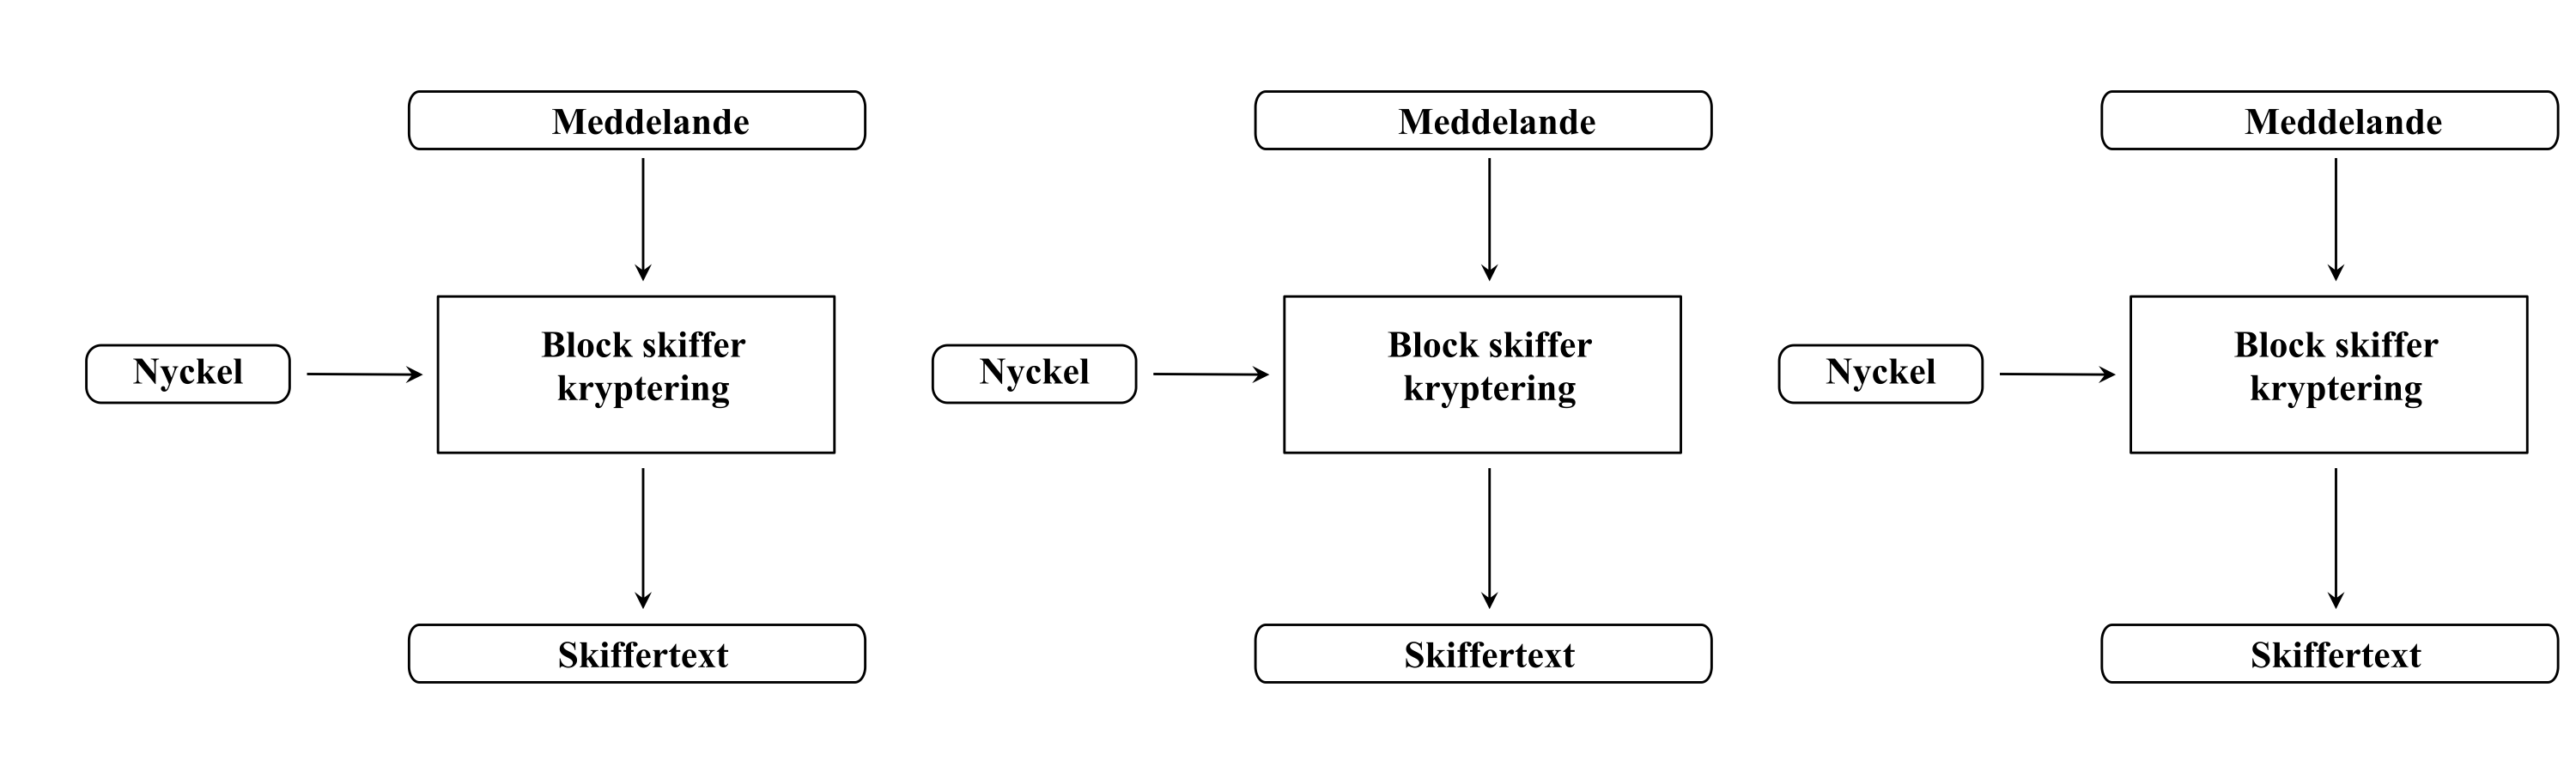
\includegraphics[width=\textwidth]{ECB Kryptering.png}
    \caption{\acrlong{ecb} kryptering}
    \label{fig:ecb-mode-enc}
\end{figure}

Figur \ref{fig:ecb-mode-dec} visar istället hur \acrshort{ecb} fungerar vid
dekryptering, vilken är en i stort sett identisk operation med det enda undantaget
att blockchiffret körs i dekrypterings läge istället för krypterings läge.

\begin{figure}[H]
    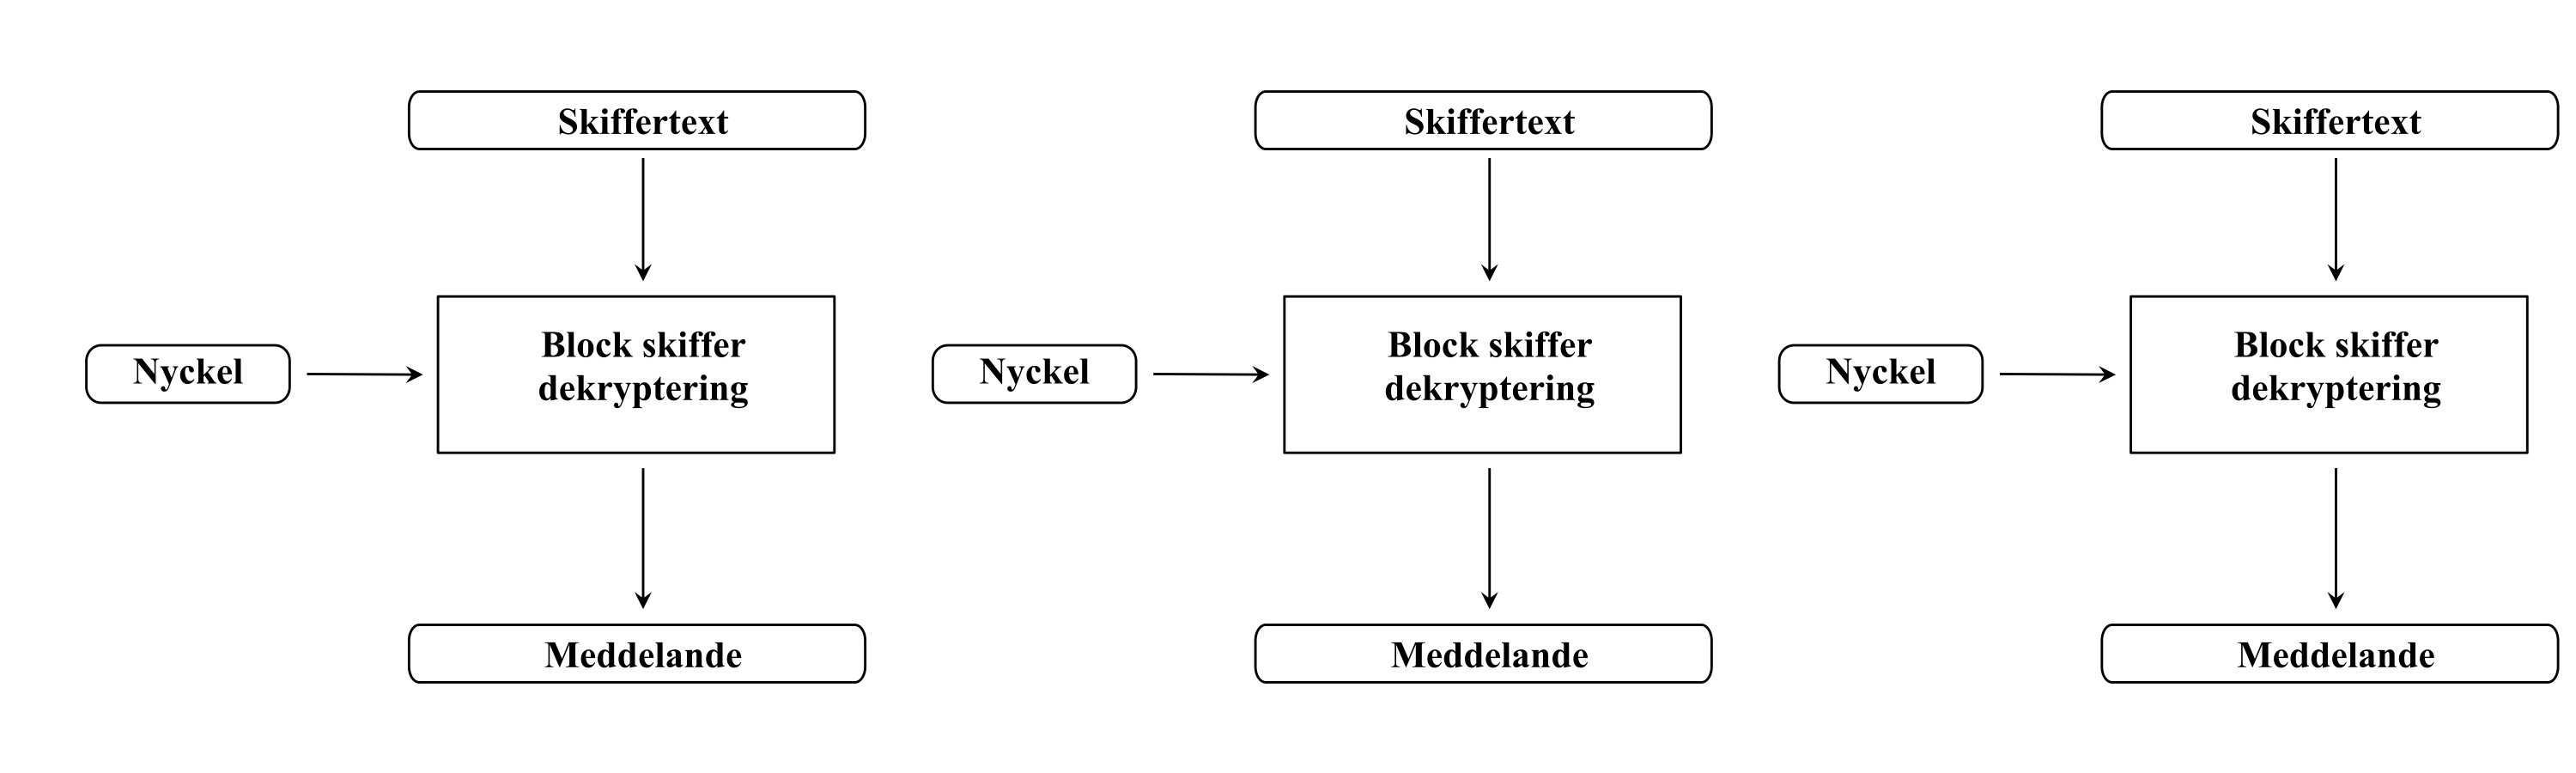
\includegraphics[width=\textwidth]{ECB Decryptering.png}
    \caption{\acrlong{ecb} dekryptering}
    \label{fig:ecb-mode-dec}
\end{figure}

På grund av \acrshort{ecb} körlägets enkelhet så finns det dock även ett ganska
stort problem med detta körläge. Det handlar om att \acrshort{ecb} inte på något
sätt förhindrar att två block med samma innehåll som krypteras inte resulterar i
ett identiskt krypterat block.\footcite{dworkin2001sp}

Vad detta innebär är att för större mängder data
är att det börjar bildas mönster i skiffertexten. Detta är något som väldigt
tydligt visar sig ifall man krypterar en bild, vilket går att se när man jämför
bilaga \ref{fig:pi-original} \& \ref{fig:pi-ecb}.
Det här faktumet är även varför \acrshort{ecb} inte betraktas som ett säkert körläge
och näst intill aldrig används i praktiken.\footcite{dworkin2001sp}

\acrshort{ecb} har däremot även sina fördelar då det bland annat kan parallelliseras
både när det gäller krypteringen och dekrypteringen. Detta samt att \acrshort{ecb}
även gör det möjligt att slumpmässigt dekryptera enskilda block av en skiffertext
utan att man behöver dekryptera hela texten.\footcite{dworkin2001sp}

\subsubsection{CBC}
\label{sec:cbc}
\acrlong{cbc}t är ett av det mest vanligen använda körlägena för många blockchiffer.
Till skillnad från \acrshort{ecb} så förhindrar \acrshort{cbc} att två block med
samma innehåll kan ge samma krypterade block. Detta gör \acrshort{cbc} genom att
lägga till ett extra steg utöver vad som finns i \acrshort{ecb}. Steget
är en \gls{xor}-operation mellan det krypterade blocket nästkommande block innan
de körs genom blockchiffer algoritmen.\footcite{dworkin2001sp}
Matematisk sett kan detta formuleras såhär:

\begin{equation}
    \label{eq:cbc-encryption}
    \begin{aligned}
        &S_i = K_n(B_i \oplus S_{i-1})\\\nonumber
        &S_0 = IV
    \end{aligned}
\end{equation}

Där $S_i$ är det krypterade blocket(skiffertexten), $B_i$ är det blocket som ska krypteras,
$K_n$ är blockskifferalgoritmen där $n$ står för nyckeln och $S_{i-1}$ är
det krypterade blocket före det blocket som ska krypteras. \acrshort{iv} är en
\acrfull{iv} som används vid krypteringen av det första blocket då det inte finns
något föregående block att använda. $i$ står för index där det första blocket har
index värdet 1. Hela den här processen kan även ses i figur \ref{fig:cbc-mode-enc}.

\begin{figure}[H]
    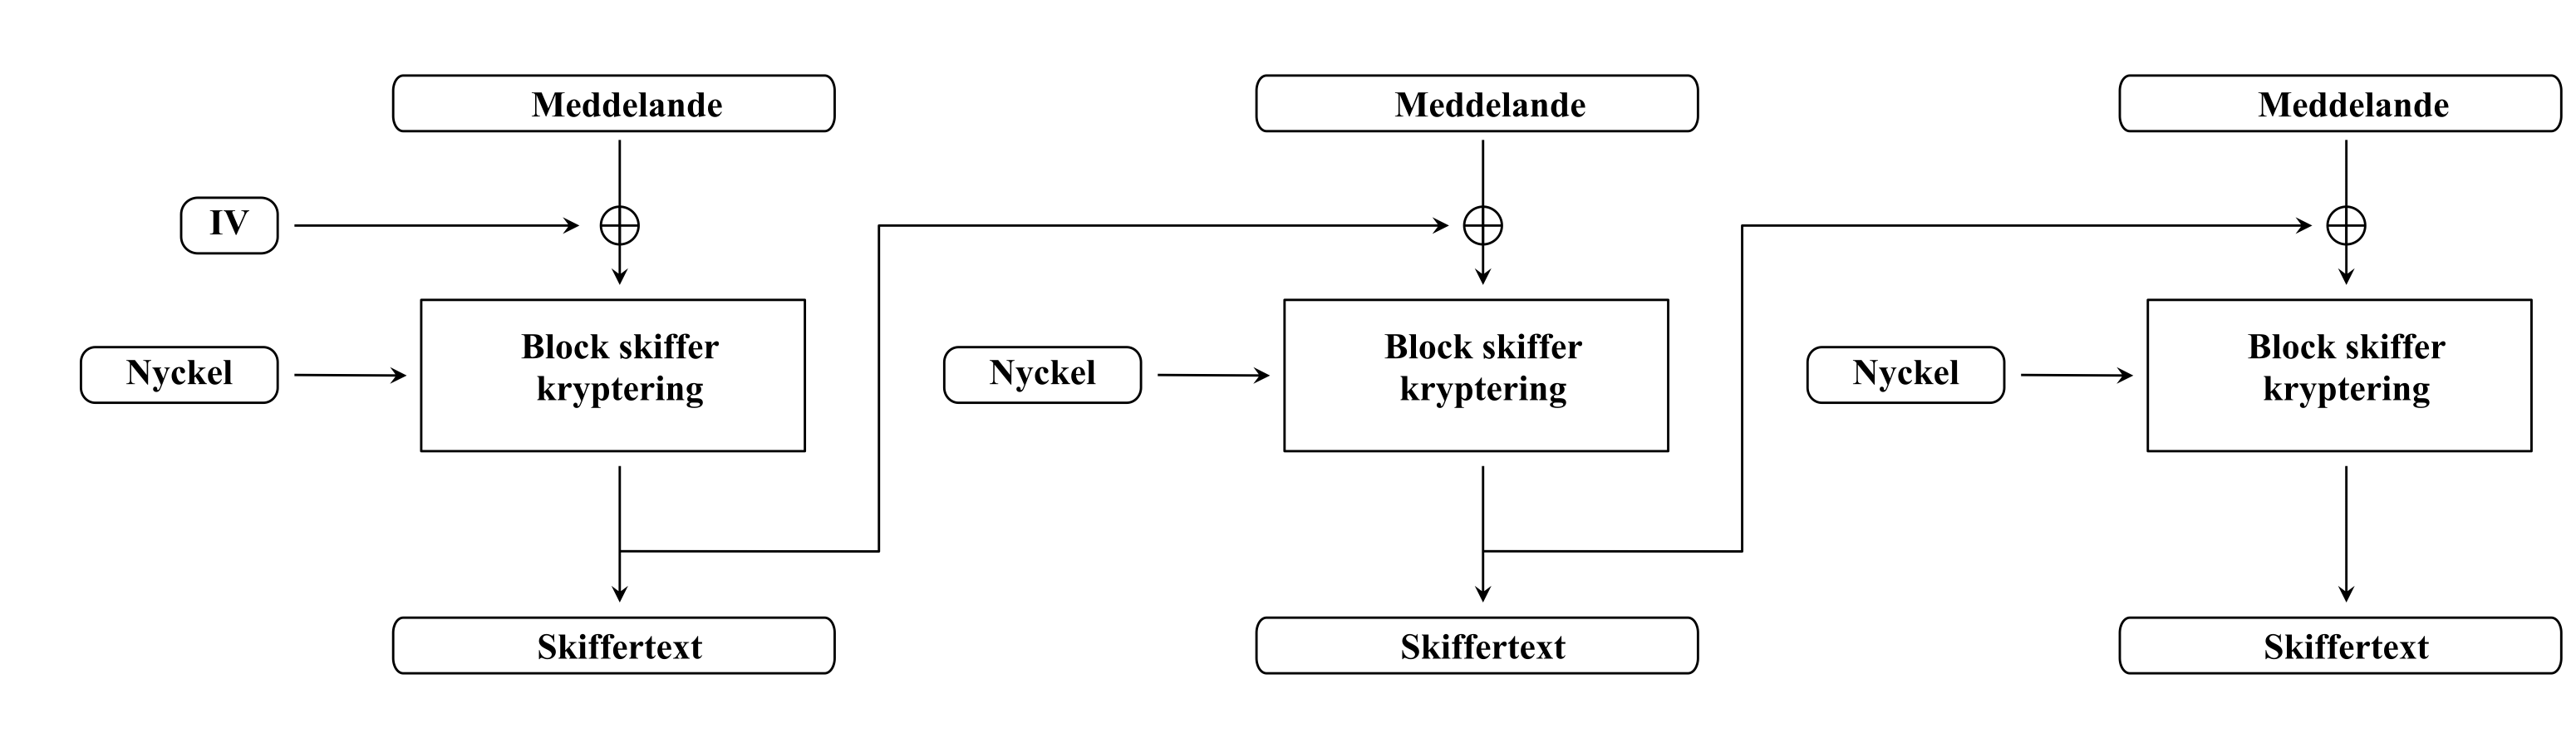
\includegraphics[width=\textwidth]{CBC Kryptering.png}
    \caption{\acrlong{cbc} kryptering}
    \label{fig:cbc-mode-enc}
\end{figure}

När det gäller dekrypterings processen för \acrshort{cbc} så bär den precis som för
\acrshort{ecb} stora likheter med krypteringsprocessen. Det två skillnaderna som
finns är att blockskifferet körs i dekrypteringsläge istället för krypterings läge.
Samt att för varje block så genomförs en \gls{xor}-operation mellan det dekrypterade
blocket och föregående block innan dekrypteringen av blocket.\footcite{dworkin2001sp}
Även detta går att både matematiskt formulera och visuellt visa såhär:

\begin{equation}
    \label{eq:cbc-decryption}
    \begin{aligned}
        &B_i = K_n(S_i) \oplus S_{i-1}\\\nonumber
        &S_0 = IV
    \end{aligned}
\end{equation}

\begin{figure}[H]
    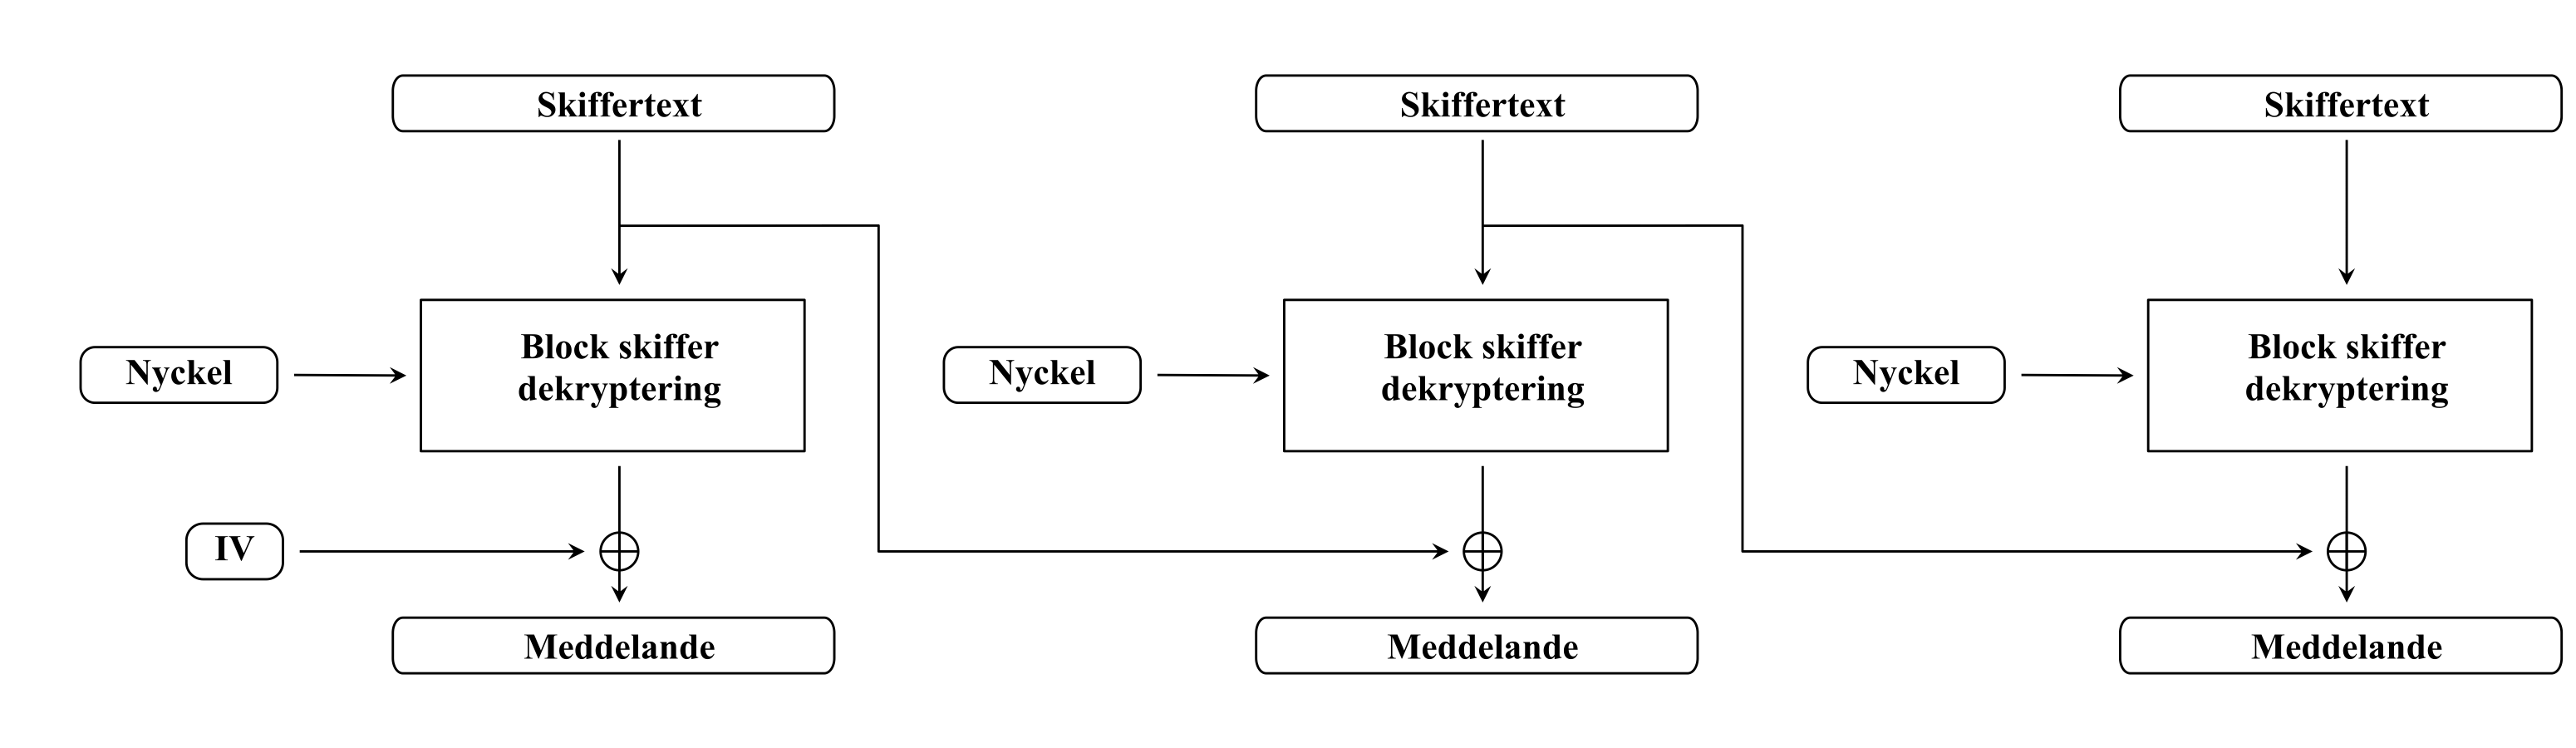
\includegraphics[width=\textwidth]{CBC Decryptering.png}
    \caption{\acrlong{cbc} dekryptering}
    \label{fig:cbc-mode-dec}
\end{figure}

Fördelarna som kommer från den extra operationen i \acrshort{cbc} till skillnad
från \acrshort{ecb} är då att varje block blir beroende av föregående block.
Detta innebär att dom mönster som kunde dyka upp i \acrshort{ecb} inte längre
kan uppstå, vilket då gör \acrshort{cbc} till ett mer säkert körläge än \acrshort{ecb}.
Dock kräver \acrshort{cbc} en ytterligare faktor för att se till så att inte olika meddelanden
kan ge samma krypterade block. Därav så krävs en \acrfull{iv} som används vid första
blocket.\footcite{dworkin2001sp}

\acrshort{cbc} är dock inte perfekt och har i sig också några nackdelar. Där ibland
exempelvis det faktum att en inkorrekt \acrshort{iv} leder till att det första blocket
inte kan dekrypteras korrekt, detta påverkar dock inte det resterande blocken. På grund
av det så kan man exempelvis lösa problemet genom att första blocket bara innehåller
någon typ av fyllnad, vilket då gör dekrypteringen möjlig utan tillgång till \acrshort{iv}.\footcite{dworkin2001sp}

Utöver detta så begränsas även \acrshort{cbc} till att bara gå att parallellisera under
dekrypteringen och inte krypteringen, vilket är en konsekvens av att varje block i \acrshort{cbc}
är beroende av föregående block. \acrshort{cbc} behåller dock fortfarande möjligheten
som \acrshort{ecb} har att slumpmässigt dekryptera enskilda block utan att behöva
dekryptera hela skiffertexten.\footcite{dworkin2001sp}

\subsubsection{OFB}
\label{sec:ofb}
\acrlong{ofb} är ett ytterligare körläge som skiljer sig en del från \acrshort{ecb}
och \acrshort{cbc} som redan presenterats. Den största skillnaden från de andra
körlägena är att \acrshort{ofb} inte använder blockskifferalgoritmen för att kryptera
eller dekryptera blocken. Istället så körs \acrshort{iv} genom blockskifferalgoritmen
och den resulterande \gls{keystream} tillförs sedan genom en \gls{xor}-operation till
blocket som ska krypteras eller dekrypteras.\footcite{dworkin2001sp}

Tack vare \gls{xor}-operationens symmetriska natur så är både krypteringen och
dekrypteringen av \acrshort{ofb} identisk, vilket även visas i figur \ref{fig:ofb-mode-enc}
\& \ref{fig:ofb-mode-dec}:

\begin{figure}[H]
    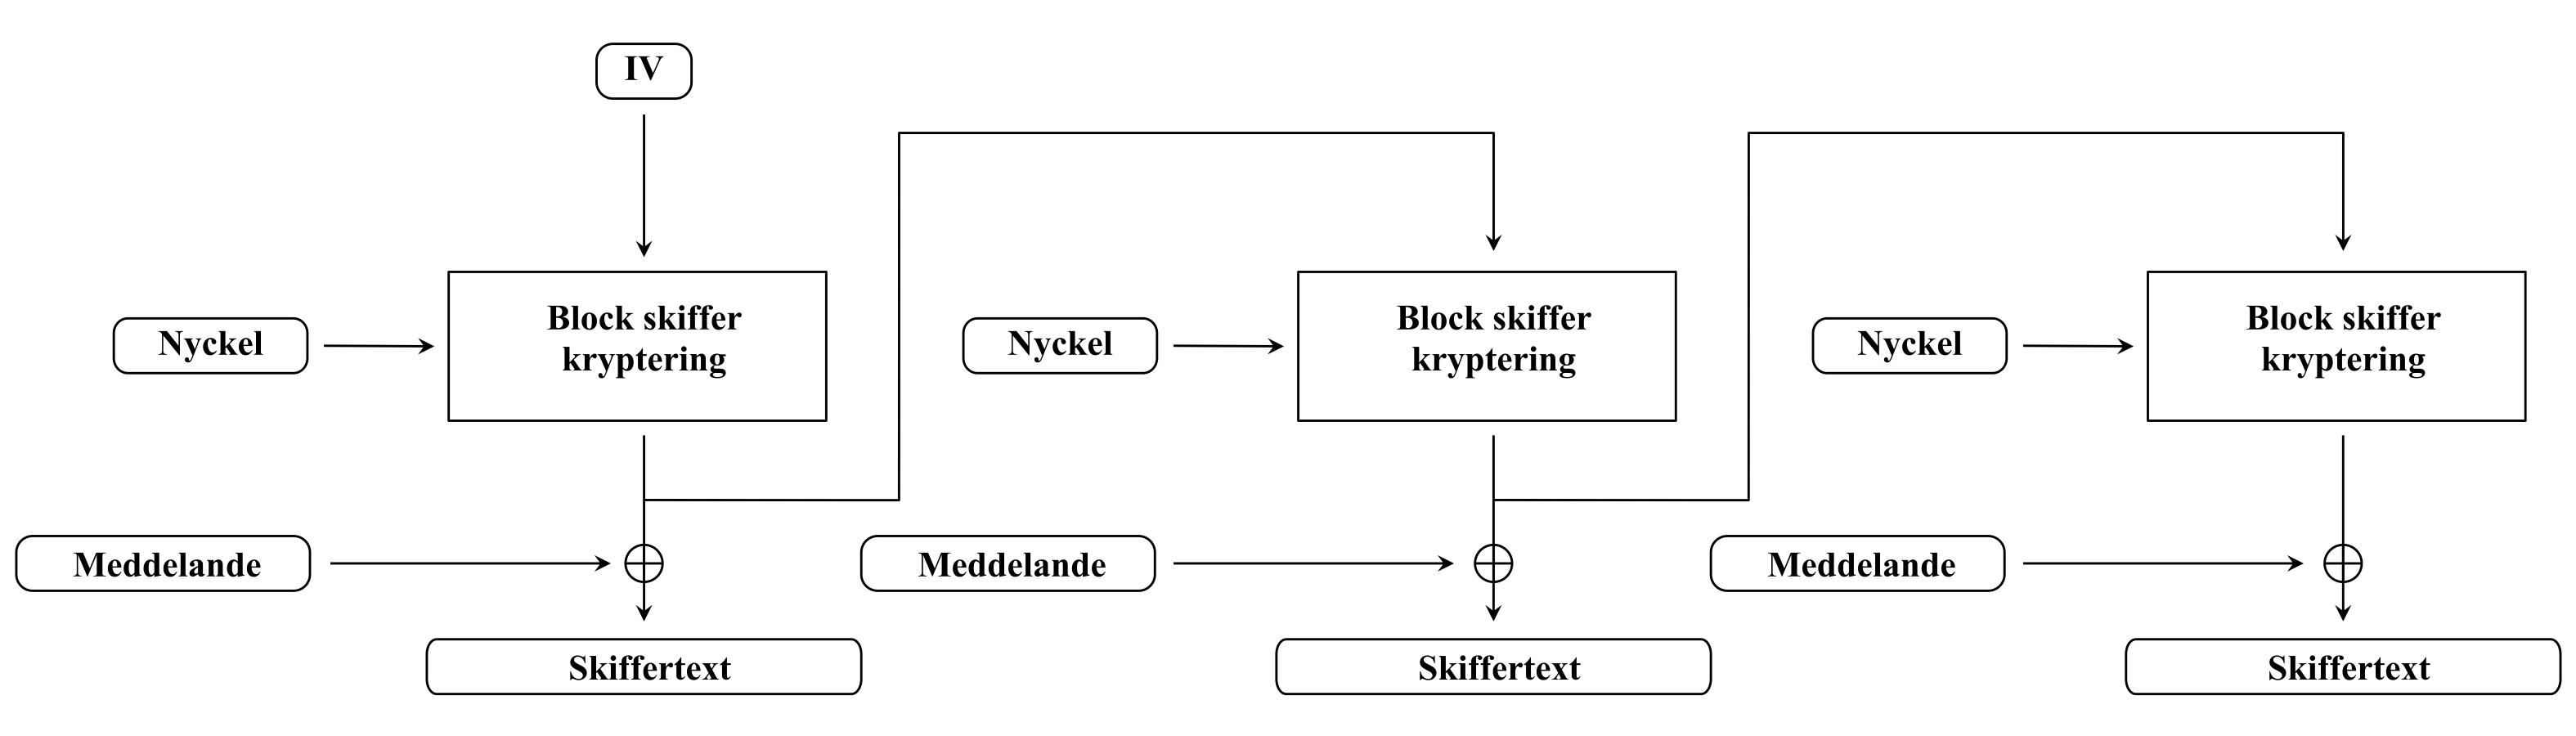
\includegraphics[width=\textwidth]{OFB Kryptering.png}
    \caption{\acrlong{ofb} kryptering}
    \label{fig:ofb-mode-enc}
\end{figure}

\begin{figure}[H]
    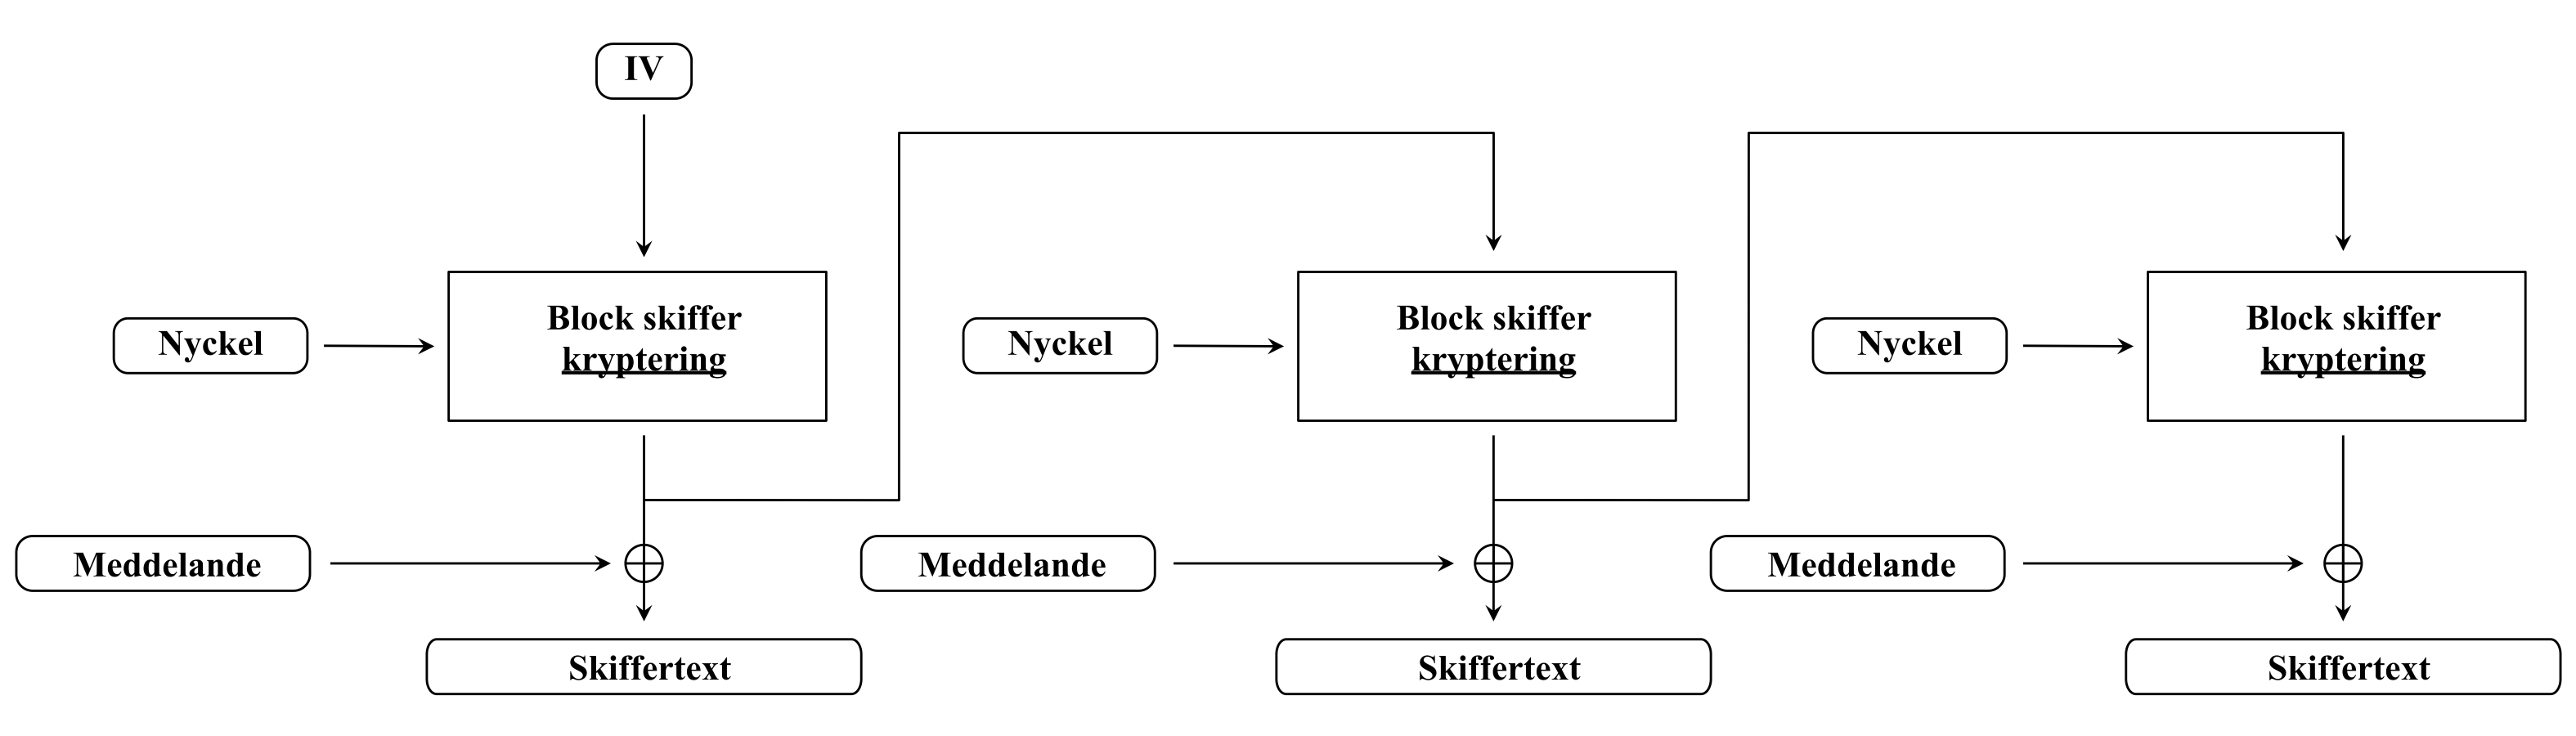
\includegraphics[width=\textwidth]{OFB Decryptering.png}
    \caption{\acrlong{ofb} dekryptering}
    \label{fig:ofb-mode-dec}
\end{figure}

Utöver detta kan man även matematiskt beskriva \acrshort{ofb}, vilket visas i ekvationerna nedan:

\begin{equation}
    \label{eq:ofb-encryption}
    \begin{aligned}
        &S_i = B_i \oplus O_i\\\nonumber
        &B_i = S_i \oplus O_i\\
        &O_i = K_n(I_i)\\
        &I_i = O_{i-1}\\
        &I_0 = IV
    \end{aligned}
\end{equation}

Här visas \acrshort{ofb} körläget matematiskt där $S_i$ är det krypterade blocket,
$B_i$ är blocket som ska krypteras och $I_0$ är \acrshort{iv}. Men här finns Även
$O_i$ som man kan säga är själva \gls{keystream}en som används för att kryptera eller
dekryptera blocket. $O_i$ i sin tur bygger då på att $O_{i-1}$ körs genom blockskifferalgoritmen
igen och sedan används för nästa blocks kryptering.

På grund av att \acrshort{ofb} är utformat på det här sättet och att själva blocken som
ska krypteras inte används fram till sista steget så är det möjligt att genomföra blockskifferoperationerna
i förväg, vilket gör det möjligt att även parallellisera \acrshort{ofb}. Dock
kan \acrshort{ofb} inte parallelliseras ifall man inte gör blockskifferoperationerna
i förväg. Utöver detta saknar även \acrshort{ofb} möjligheten att slumpmässigt dekryptera
enskilda block utan att behöva dekryptera hela skiffertexten.\footcite{dworkin2001sp}

\section{Symetrisk \& Asymmetrisk Kryptering}
\label{sec:symmetric-asymmetric-encryption}
Symmetrisk och asymmetrisk kryptering handlar om hur nycklar används i olika
krypteringsalgoritmer. För symmetriska krypteringsalgoritmer så betyder detta
att samma nyckel är vad som används för både kryptering och dekryptering. Medans
asymmetrisk kryptering bygger på att man använder olika nycklar för kryptering och
dekrypterings processerna.\footfullcite{symencrypt}

De symmetriska krypteringsalgoritmernas huvudsakliga nackdel ligger i det faktum att
de krävs en delad känd nyckel mellan båda parter. Detta är något som asymmetriska
krypteringsalgoritmer inte behöver, vilket har lett till att man ofta använder
asymmetriska krypteringsalgoritmer för att sköta nyckelutbytet för det symmetriska
krypteringsalgoritmerna. Anledningen till detta är att det symmetriska krypteringsalgoritmerna
ofta är bättre för större datamängder då dom bland annat behöver mycket
kortare nyckellängder.\footcite{symencrypt}

Exempel på symmetriska krypteringsalgoritmer är bland annat \acrshort{aes} och
\acrshort{des} varav \acrshort{aes} kommer förklaras djupare senare i denna rapport.\footcite{symencrypt}
Exempel på asymmetriska krypteringsalgoritmer är bland annat \gls{rsa}.\footfullcite{rsa-ref}

\section{AES}
\label{sec:aes}

Som nämnts tidigare i \nameref{sec:aes-uppkomst} bygger \acrshort{aes}-standarden på en variant av Rijndael \nameref{sec:blockskiffer} algoritmen
skapad av Vincent Rijmen och Joan Daemen. \acrshort{aes} är en symmetrisk \nameref{sec:blockskiffer}krypteringsalgoritm som utformades för att ersätta
\acrshort{des} som då var den dominerande krypteringsalgoritmen. \acrshort{aes} är en av det mest använda krypteringsalgoritmerna idag
och används bland annat i säkerhetsprotokoll så som \acrfull{wpa2}\footfullcite{wpa2_ref}. \acrshort{aes} går att dela upp i tre olika varianter
som alla är baserade på samma grundläggande struktur. Dessa varianter är \acrshort{aes}-128bit, \acrshort{aes}-192bit och \acrshort{aes}-256bit som huvudsakligen
skiljer sig från varandra när det kommer till längden av krypteringsnyckeln samt antalet rundor som genomförs i algoritmens krypterings process.\footfullcite{aes_wiki}

Även själva algoritmen kan delas upp i ett antal olika delar som alla har olika syften. Dessa delar är \nameref{sec:aes-addroundkey}, \nameref{sec:aes-subbytes}, \nameref{sec:aes-shiftrows},
\nameref{sec:aes-mixcolumns} och \nameref{sec:aes-key-expansion} som alla kommer att förklaras mer detaljerat i det följande sektioner. \nameref{sec:aes-key-expansion} delen kan även
delas upp ytterligare i tre olika varianter 128bit, 192bit och 256bit beroende på vilken av det tre \acrshort{aes} varianterna som används.\footfullcite{daemen1999aes}

Utöver detta så bygger \nameref{sec:aes-key-expansion} på tre operationer vilka är \nameref{sec:aes-subword}, \nameref{sec:aes-rotword} och
\nameref{sec:aes-rcon} som också kommer att förklaras mer detaljerat i det följande sektioner.\footcite{aes_wiki} För att förstå vissa av dessa delar
så kommer det däremot krävas en förklaring av både \nameref{sec:aes-sbox} och \nameref{sec:finite-fields} först.\footcite{daemen1999aes}

\subsection{Finite Fields}
\label{sec:finite-fields}
Inom bland annat matematiken och datorvetenskapen finns begreppet Finite Fields
som även på svenska kallas för ändliga kroppar. Finite Fields är en matematisk
koncept som bland annat kan användas ifall man vill kunna utföra aritmetiska
operationer som addition, subtraktion, multiplikation och division med ett
bestämt antal element. Produkten från varje operation inom ett Finite Field
kommer då alltid att vara ett element inom samma Finite Field.\footfullcite{finitefield_wiki}

Detta är ett viktigt koncept för \acrshort{aes} då \acrshort{aes} använder sig av
Finite Fields för att utföra vissa av sina operationer. Där anledningen till behovet
ligger i att \acrshort{aes} jobbar på bytenivå vilket innebär att alla operationer
som utförs måste resultera i ett värde som är mellan 0 och 255. \acrshort{aes} Finite Field
kan då med detta skrivas som $GF(2^8)$ där $GF$ står för Galios Field vilket är
en annan benämning på Finite Fields.\footcite{finitefield_wiki} För en mer grundlig matematisk förklaring av Finite Fields så kan man läsa vidare i rapporten
\citetitle{boman2016andliga} av \citeauthor{boman2016andliga}.\footfullcite{boman2016andliga}

\subsection{AES S-Box}
\label{sec:aes-sbox}
\acrshort{aes} använder sig av en så kallad S-Box eller med andra ord substitutions box
för en del av sina operationer. S-Boxen används huvudsakligen för att byta ut värden
i \nameref{sec:aes-key-expansion}s delen av \acrshort{aes} algoritmen samt i
\nameref{sec:aes-subbytes}.\footfullcite{sbox_wiki}

S-boxen består av 256 olika värden som alla är unika och som alla är mellan 0 och 255.
Värdena i S-boxen är ordnade i en lista och värdenas position i listan används som
index för att kunna hitta ett värde i S-boxen. När S-boxen används för att byta ut
ett värde så används det värde som ska bytas ut som indexvärde för att kunna hitta
rätt värde i S-boxen.\footcite{sbox_wiki}

\acrshort{aes} S-box genereras med hjälp av \acrshort{aes} Finite Field {$GF(2^8)$}.
Själva S-boxen är konstant genom hela \acrshort{aes} algoritmen och kan därför
vara en attackvektor för olika försök till att bryta krypteringen. På grund av
detta så finns det även användningar av dynamiska S-boxar som kan genereras
utifrån en viss nyckel och skapar då ytterligare ett lager av säkerhet.\footfullcite{singh2017analysis}

\acrshort{aes} har två olika S-boxar varav den ena är en invers av den andra.
Detta så att operationen går att utföra i båda riktningarna, vilket gör dekryptering
av data möjlig.\footcite{sbox_wiki} Dessa två S-boxar går att se nedan i figur \ref{fig:aes-sbox} där
värdena är representerade i \gls{hexadecimal} tal.

\begin{figure}[H]
    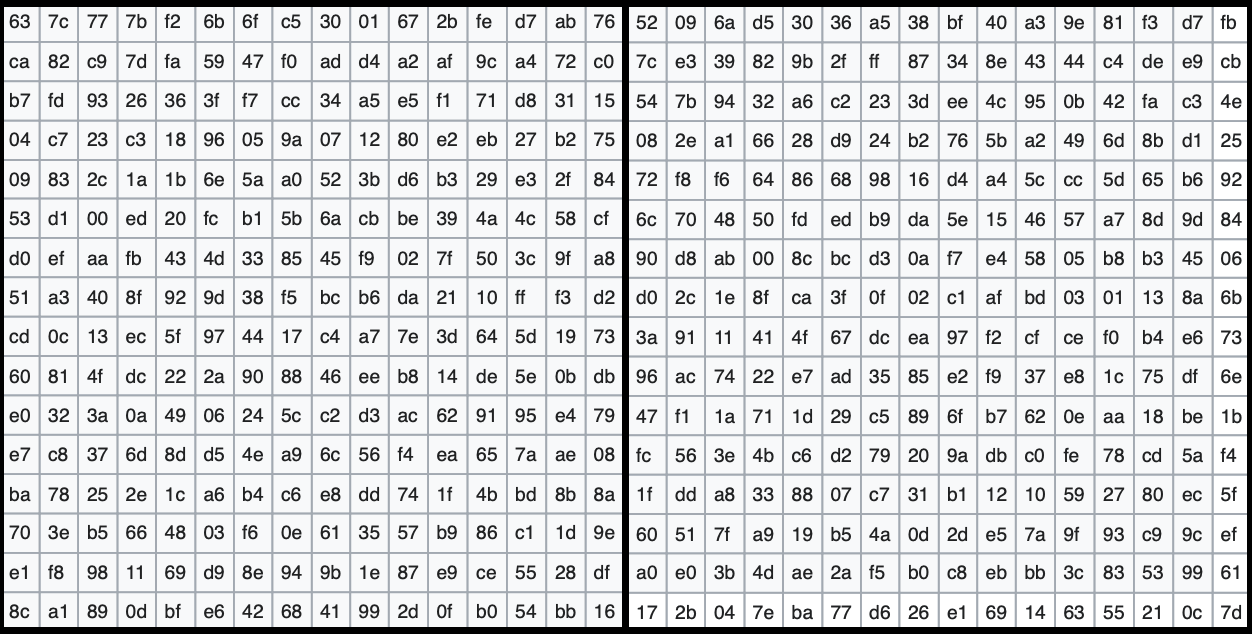
\includegraphics[width=\textwidth]{S-box.png}
    \caption{\acrshort{aes} S-box (Den vänstra matrisen) \& Invers S-box (Den högra matrisen)}
    \label{fig:aes-sbox}
\end{figure}

\subsection{Struktur}
\label{sec:aes-structure}
\acrshort{aes} är baserad på en design princip kallad \gls{SP-network} och byggs huvudsakligen upp av fyra olika steg som alla utförs på en matris av 16 \glspl{byte}. Dessa fyra steg är
\nameref{sec:aes-subbytes}, \nameref{sec:aes-shiftrows}, \nameref{sec:aes-mixcolumns} och
\nameref{sec:aes-addroundkey}, vilket visas i figur \ref{fig:round-function}. Stegen utförs antingen 10, 12 eller 14 gånger, vilket brukar kallas för rundor.
\footcite{daemen1999aes}

Beroende på vilken nyckel som används krävs olika antal rundor.
En 128bit nyckel kommer att kräva 10 rundor, en 192bit nyckel kommer att kräva 12 rundor och en 256bit nyckel kommer att kräva 14 rundor.
Detta brukar man se som det tre olika krypterings lägena \acrshort{aes}-128bit \acrshort{aes}-192bit och \acrshort{aes}-256bit som
då är det tre olika nyckelstorlekarna som \acrshort{aes} stödjer.\footcite{daemen1999aes}

\acrshort{aes}-algoritmen har en fast block storlek på 128bit vilket innebär att
det alltid kommer att vara 16 \glspl{byte} som krypteras åt gången. Absolut först genomförs
en initial \nameref{sec:aes-addroundkey} där den första rundnyckeln används.
Sedan genomförs 9, 11 eller 13 identiska rundor. Den sista rundan skiljer sig däremot från det andra
på så sätt att man hoppar över sista \nameref{sec:aes-mixcolumns} då den inte får någon betydelse ur ett
kryptografiskt perspektiv för den slutliga skiffer texten.\footcite{daemen1999aes}

\begin{wrapfigure}{r}{0.5\textwidth}
    \centering
    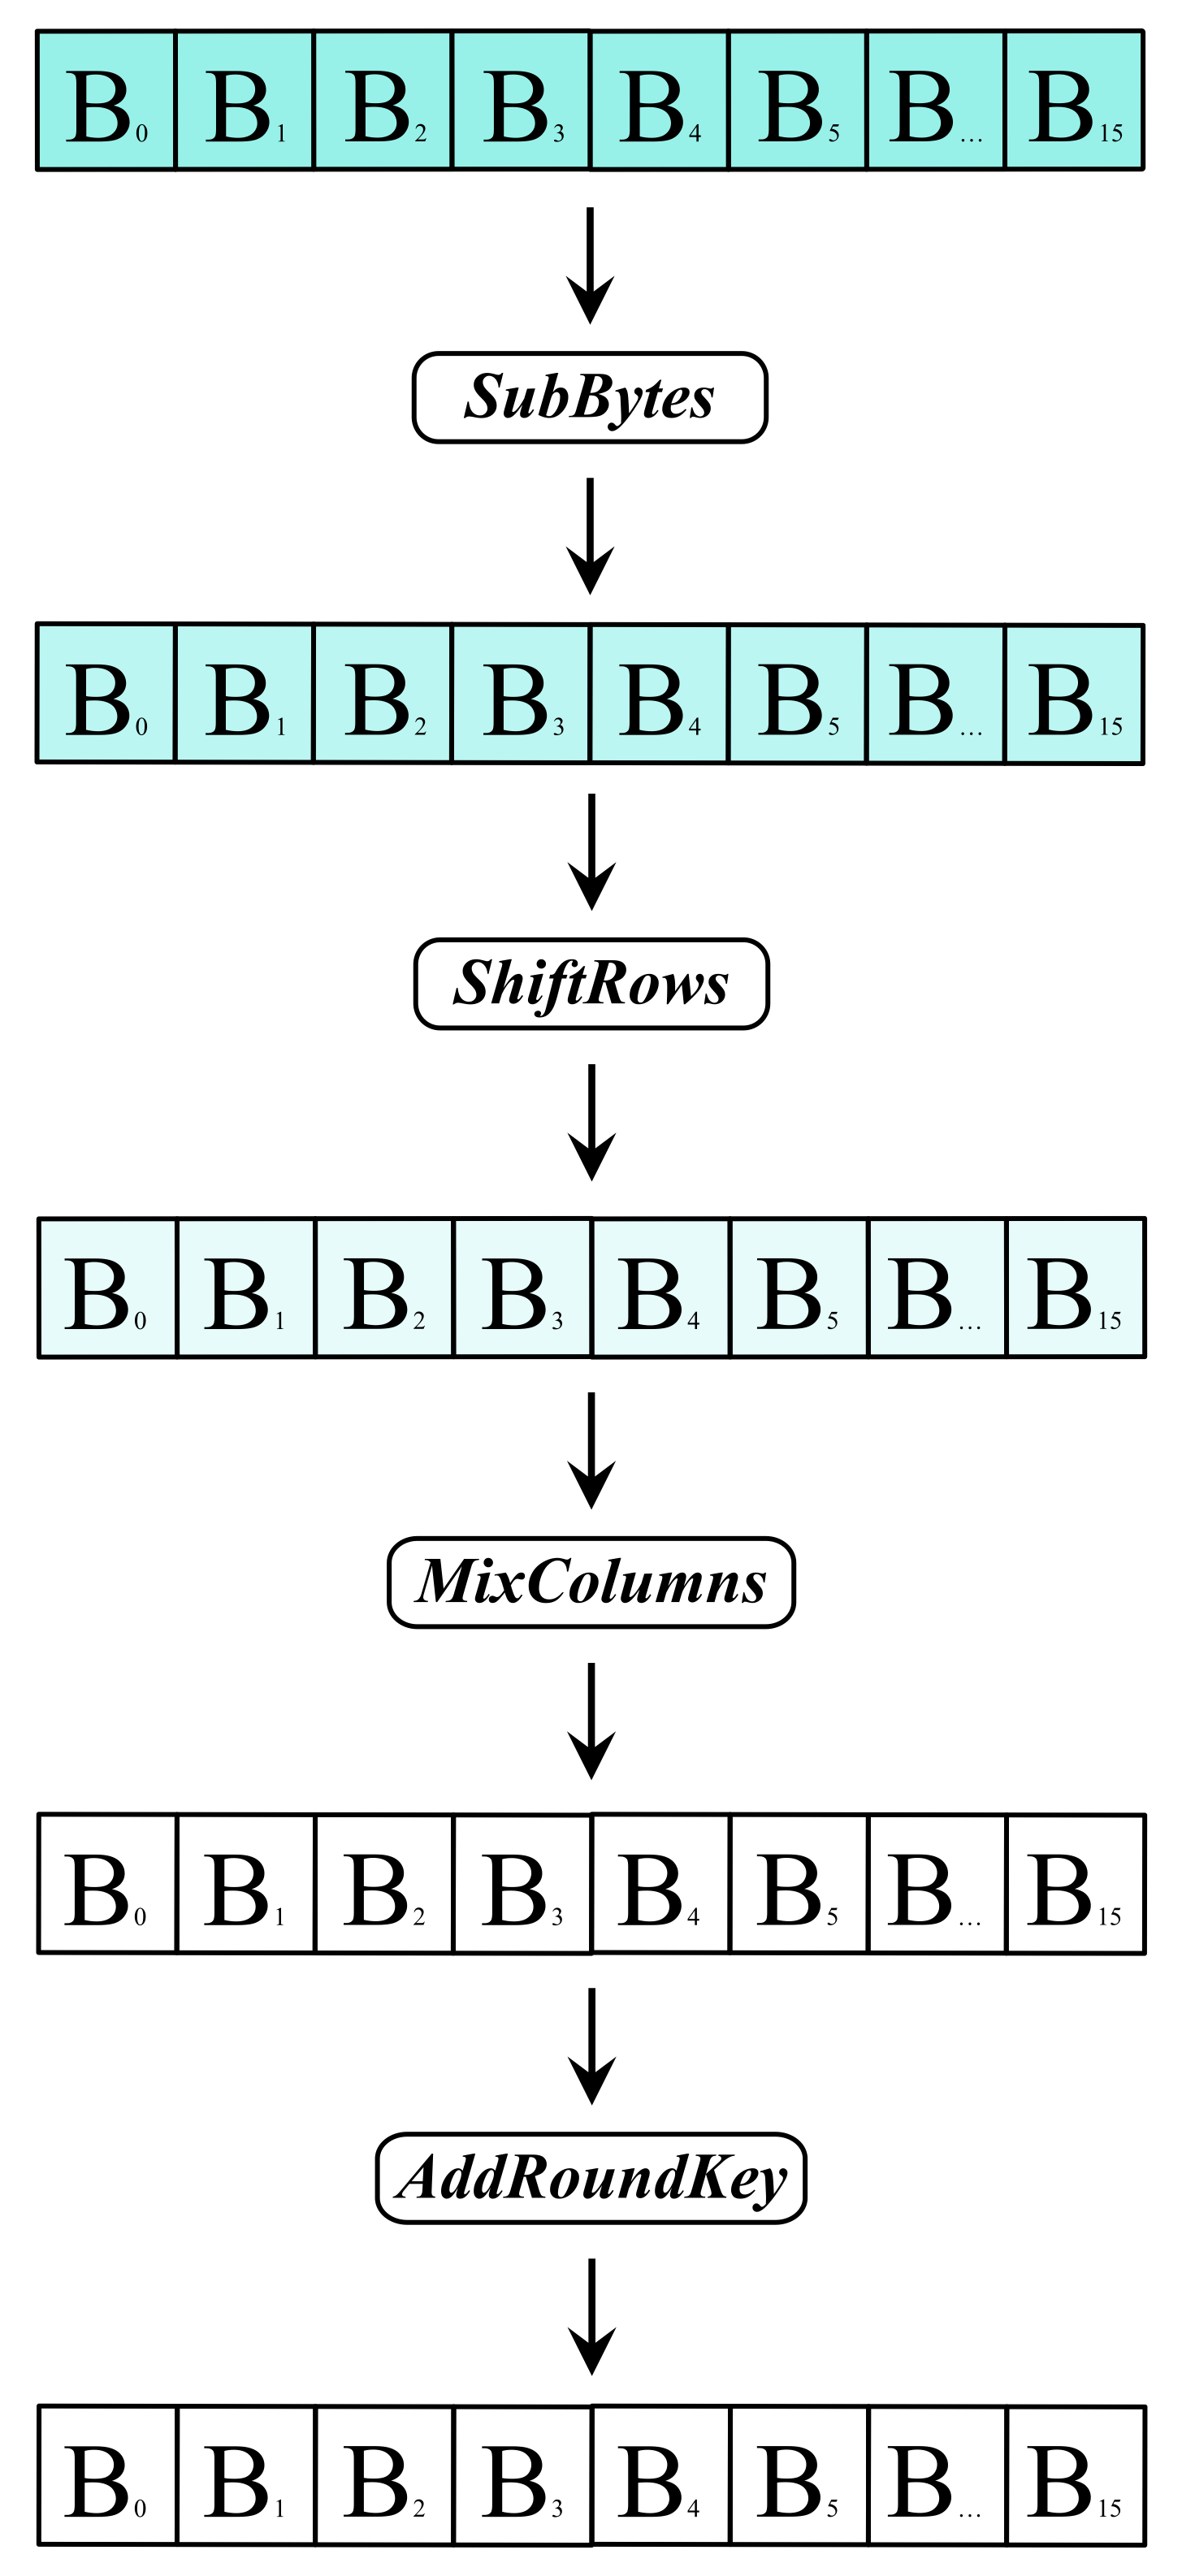
\includegraphics[width=0.5\linewidth]{Vanlig runda.png}
    \caption{Vanlig runda}
    \label{fig:round-function}
\end{wrapfigure}

En vanlig runda består av följande steg:

\begin{enumerate}
    \item \nameref{sec:aes-subbytes}
    \item \nameref{sec:aes-shiftrows}
    \item \nameref{sec:aes-mixcolumns}
    \item \nameref{sec:aes-addroundkey}
\end{enumerate}

Den sista rundan ser istället ut på följande sätt:

\begin{enumerate}
    \item \nameref{sec:aes-subbytes}
    \item \nameref{sec:aes-shiftrows}
    \item \nameref{sec:aes-addroundkey}
\end{enumerate}

Utifrån detta kan man se att nyckeln används flera gånger under själva krypteringsprocessen av ett block.
För att varje runda ska få en unik nyckel så genomförs en \nameref{sec:aes-key-expansion}s operation
som genererar en nyckel för varje runda utifrån den ursprungliga nyckeln. Detta för att samma nyckel
inte ska användas flera gånger vilket skulle göra det enklare att bryta krypteringen.\footcite{daemen1999aes}

\nameref{sec:aes-key-expansion}en är en operationen som genomförs före själva krypteringsstadiet påbörjas
och genererar en lista med nycklar för varje runda. Antalet nycklar beror av nyckellängden som även bestämmer antalet rundor.
För dekryptering så sker liknande rundor av operationer som för krypteringen fast
i en lite annorlunda ordning samt med den motsatta operationen till \nameref{sec:aes-shiftrows} \& \nameref{sec:aes-mixcolumns}.\footcite{daemen1999aes}

En vanlig runda för dekryptering ser ut på följande sätt:

\begin{enumerate}
    \item \nameref{sec:aes-addroundkey}
    \item \nameref{sec:aes-invers-mixcolumns}
    \item \nameref{sec:aes-invers-shiftrows}
    \item \nameref{sec:aes-subbytes}
\end{enumerate}

Anledningen till att \nameref{sec:aes-addroundkey} och \nameref{sec:aes-subbytes} inte kräver någon direkt motsatt funktion har och göra med hur dessa operationer
är uppbyggda. För \nameref{sec:aes-addroundkey} så är det på grund av \gls{xor}-operationens linjära egenskaper som innebär att den är sin egen invers.
Detta eftersom ifall man tar och genomför \gls{xor}-operationen med samma nyckel två gånger så kommer man tillbaka till ursprungsvärdet.

När det gäller \nameref{sec:aes-subbytes}
så handlar det istället om att det helt enkelt är en substitution utifrån en \nameref{sec:aes-sbox}, vilket då betyder att det som krävs för att genomföra den motsatta operationen
blir att använda den motsatta \nameref{sec:aes-sbox}en.\footcite{daemen1999aes}

Både krypterings- och dekrypteringsstrukturen som nu beskrivits kan implementeras i exempelvis \gls{python} kod som visas i figur \ref{fig:encryption-rounds-function} \& \ref{fig:decryption-rounds-function}.

\begin{figure}[H]
    \centering
    \begin{python}
    # Performs the encryption rounds on the input data matrix
    # This function is used for the encryption of data matrixes
    # using the expanded keys.
    def encryption_rounds(data, round_keys, nr):
        # Inizial add round key
        data = np.bitwise_xor(data, round_keys[0])

        # Rounds 1 to 9 or 1 to 11 or 1 to 13
        # Here each step in one round is performed in a sequence n times
        # where n is the number of rounds minus the last round.
        for i in range(1, (nr - 1)):
            # Sub bytes
            data = sub_bytes(data, subBytesTable)
            # Shift rows
            data = shift_rows(data)
            # Mix columns
            data = mix_columns(data)
            # Add round key
            data = np.bitwise_xor(data, round_keys[i])

        # Final round
        # Identical to the previous rounds, but without mix columns
        data = sub_bytes(data, subBytesTable)
        data = shift_rows(data)
        data = np.bitwise_xor(data, round_keys[nr - 1])

        # Returns the encrypted data
        return data

    \end{python}
    \caption{Krypterings runda funktion}
    \label{fig:encryption-rounds-function}
\end{figure}

\begin{figure}[H]
    \centering
    \begin{python}
    # Performs the decryption rounds on the input data matrix
    # This function is used for the decryption of data matrixes
    # using the expanded keys.
    def decryption_rounds(data, round_keys, nr):
        # Inizial add round key, inverse shift rows and inverse sub bytes
        data = np.bitwise_xor(data, round_keys[-1])
        data = inv_shift_rows(data)
        data = sub_bytes(data, invSubBytesTable)

        # Rounds 1 to 9 or 1 to 11 or 1 to 13
        # Here each step in one round is performed in a sequence n times
        # where n is the number of rounds minus the last round.
        for i in range(1, (nr - 1)):
            # Add round key
            data = np.bitwise_xor(data, round_keys[-(i+1)])
            # Inverse mix columns
            data = inv_mix_columns(data)
            # Inverse shift rows
            data = inv_shift_rows(data)
            # Inverse sub bytes
            data = sub_bytes(data, invSubBytesTable)

        # Final round
        # Final add round key of final round
        data = np.bitwise_xor(data, round_keys[0])

        # Returns the decrypted data
        return data

    \end{python}
    \caption{Dekrypterings runda funktion}
    \label{fig:decryption-rounds-function}
\end{figure}

\subsubsection{SubBytes-operationen} %(To be reviwed)
\label{sec:aes-subbytes}
SubBytes-operationen bygger på att varje \gls{byte} byts ut mot en korresponderande \gls{byte} från en \nameref{sec:aes-sbox} som
visas i figur \ref{fig:aes-subbytes-pic}.
Själva operationen fungerar som det ickelinjära steget i krypteringsprocessen och är därmed en viktig del av AES.\footcite{daemen1999aes}

\begin{figure}[H]
    \centering
    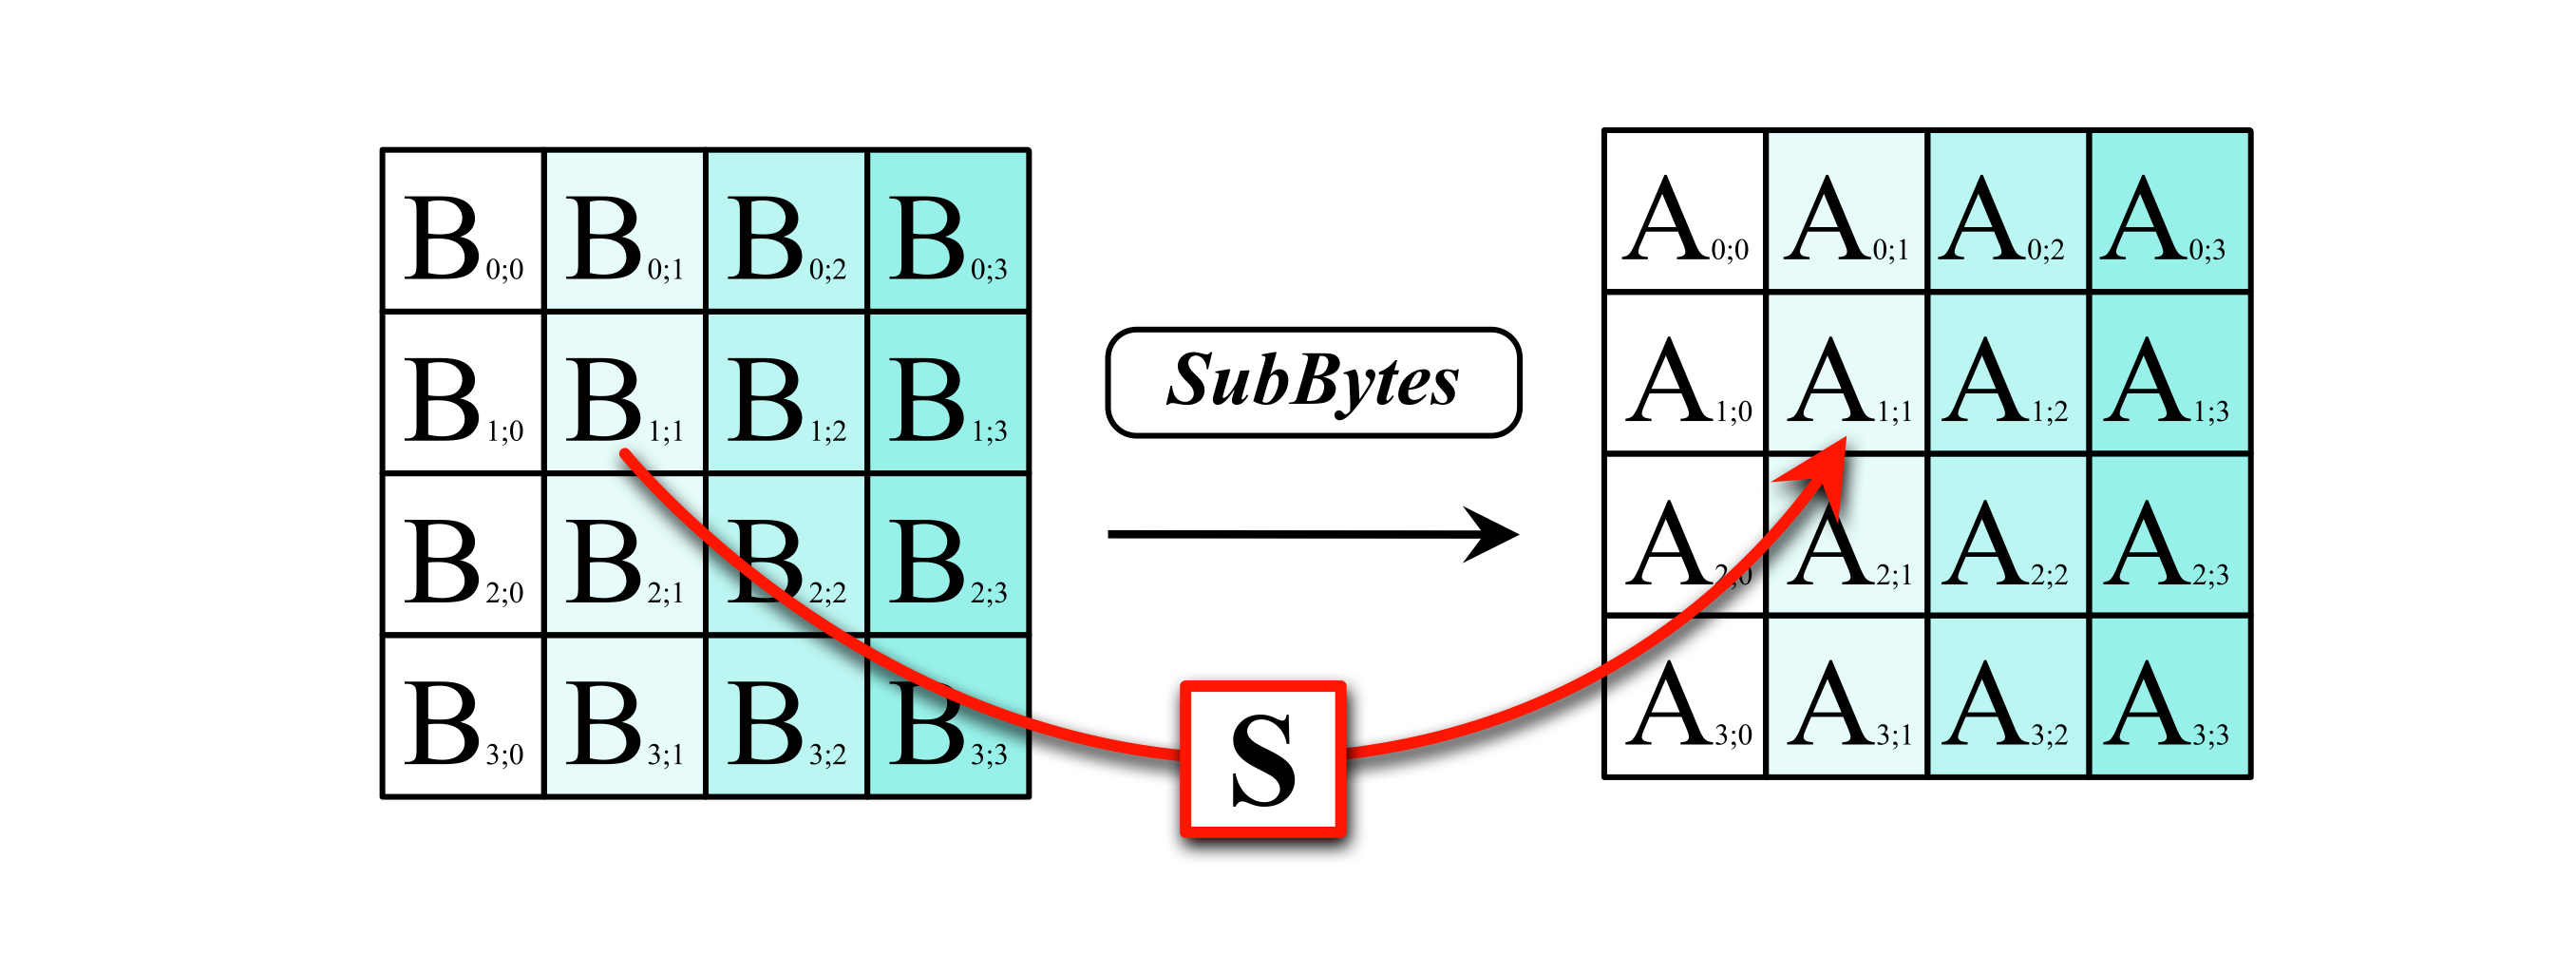
\includegraphics[width=0.7\textwidth]{SubBytes.png}
    \caption{SubBytes operationen}
    \label{fig:aes-subbytes-pic}
\end{figure}

För att genomföra den motsatta varianten av SubBytes operationen så krävs endast att man använder den motsatta \nameref{sec:aes-sbox}en,
vilket då resulterar i den ursprungliga \gls{byte}-matrisen.\footcite{daemen1999aes} Vilket visas i figur \ref{fig:aes-inverse-subbytes-pic}.

\begin{figure}[H]
    \centering
    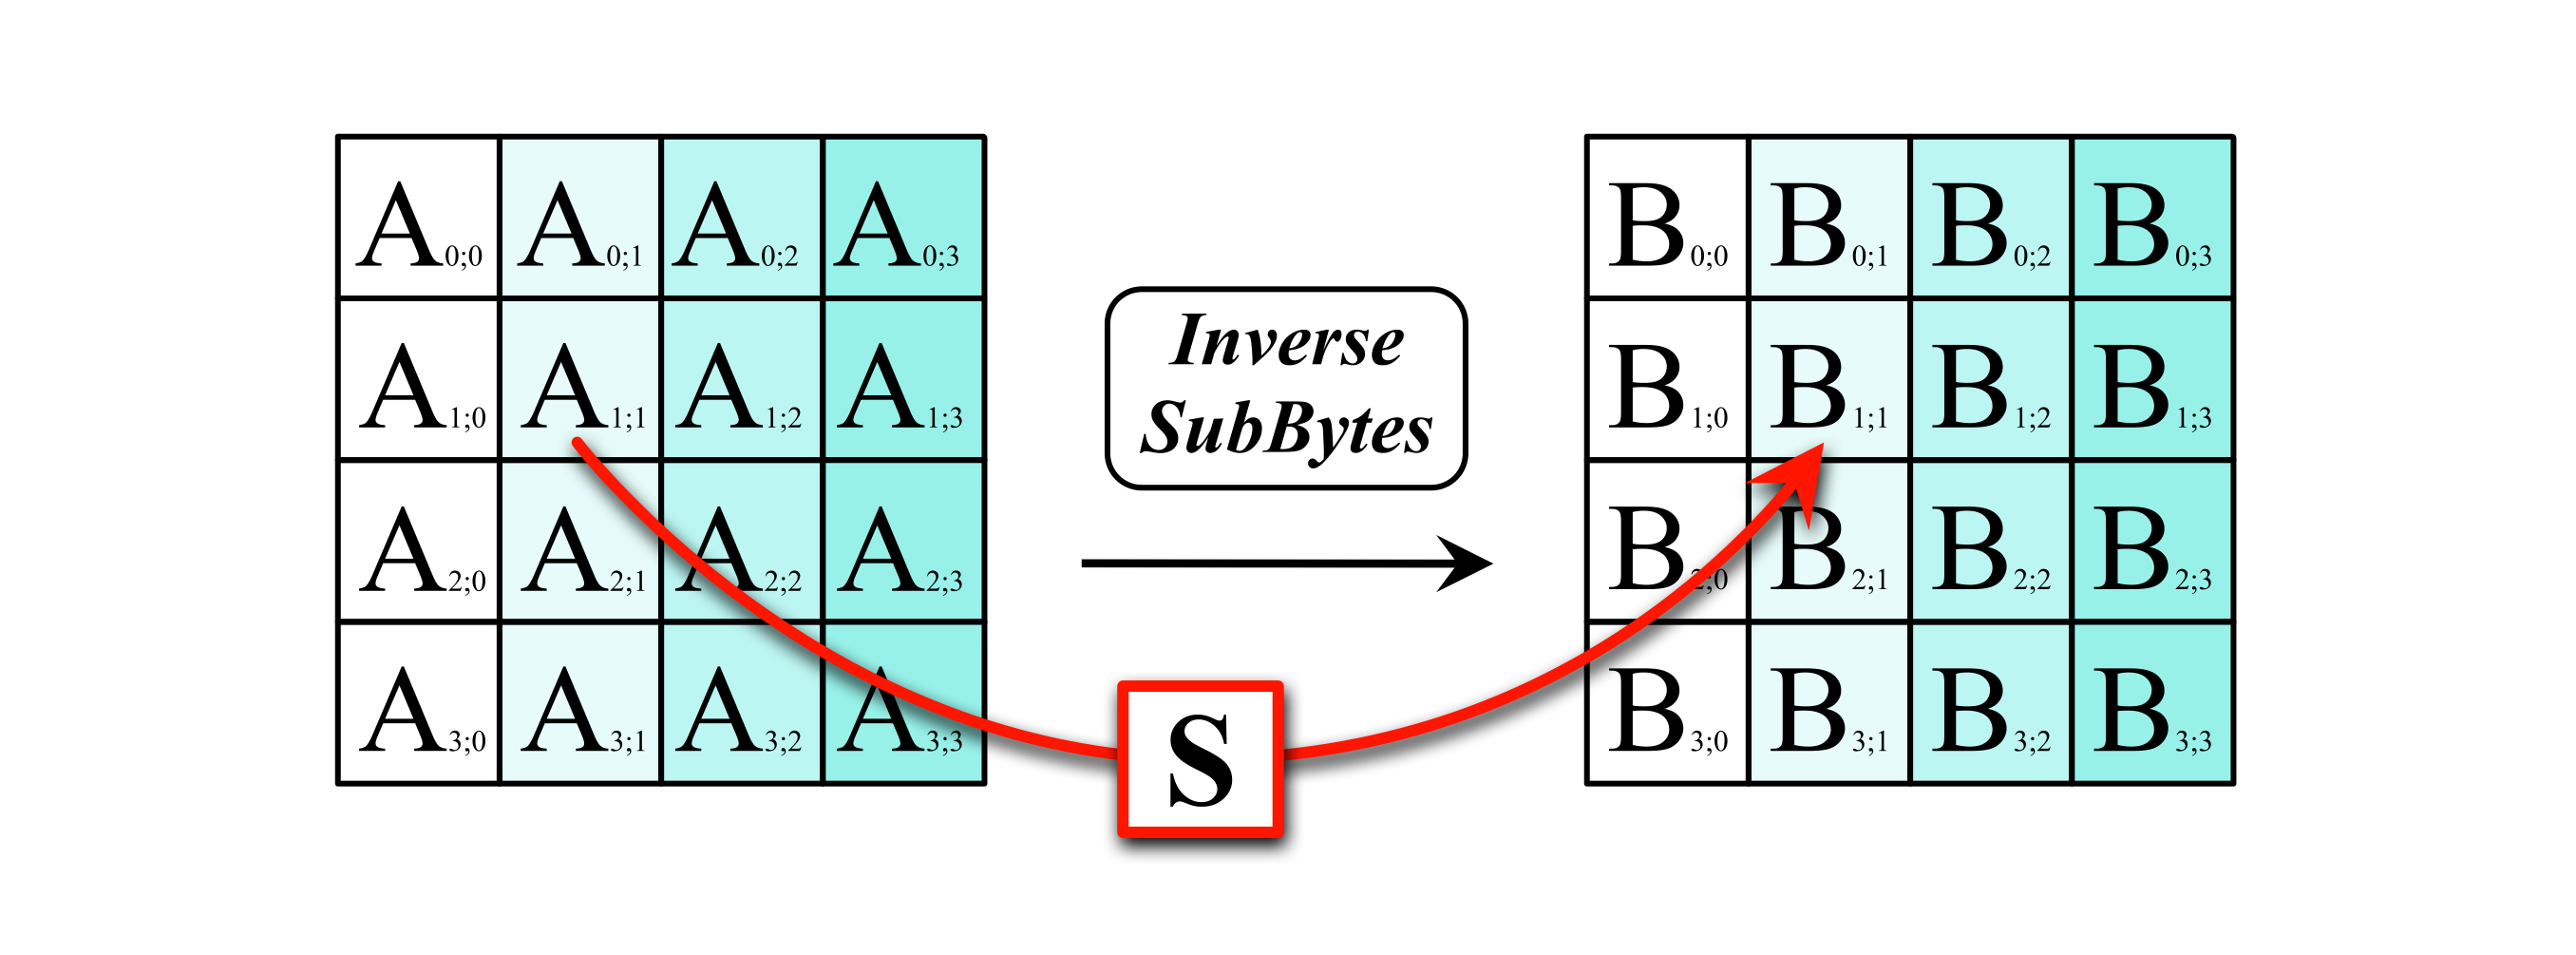
\includegraphics[width=0.7\textwidth]{Inverse-SubBytes.png}
    \caption{Inverse SubBytes operationen}
    \label{fig:aes-inverse-subbytes-pic}
\end{figure}

\subsubsection{ShiftRows operationen}
\label{sec:aes-shiftrows}

ShiftRows operationen är en operation som bygger på att varje rad i \gls{byte} matrisen förflyttas i sidled ett visst antal steg.
Första raden förflyttas 0 steg, andra raden 1 steg åt vänster, tredje raden 2 steg åt vänster och fjärde raden 3 steg åt vänster. Anledningen till att ShiftRows-steget
finns är för att kolumnerna i \gls{byte} matrisen krypteras oberoende av varandra.\footcite{daemen1999aes}

\begin{figure}[H]
    \centering
    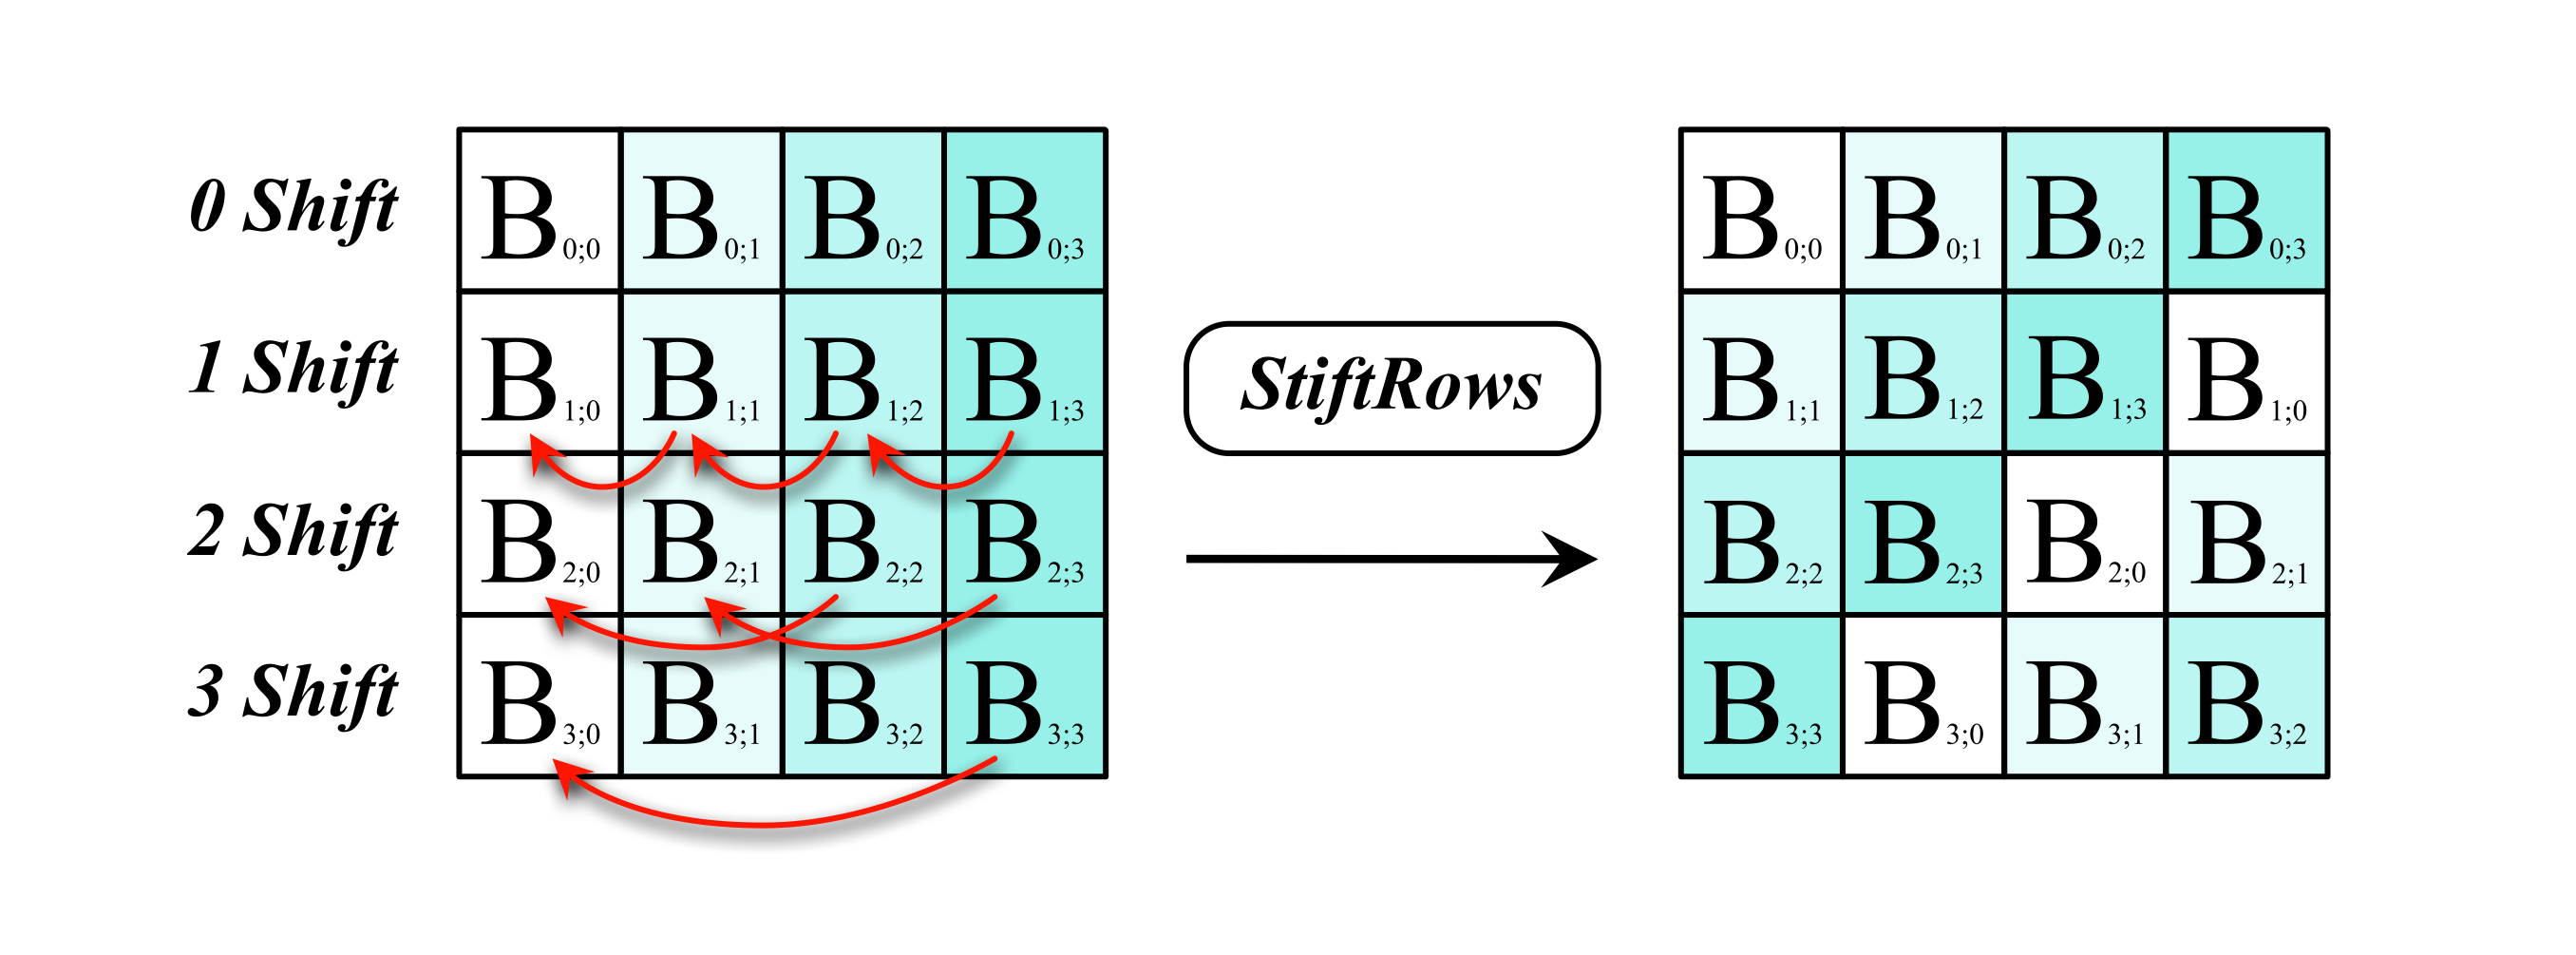
\includegraphics[width=0.7\textwidth]{ShiftRows.png}
    \caption{ShiftRows operationen}
    \label{fig:aes-shiftrows-pic}
\end{figure}

\subsubsection{Inverse ShiftRows-operationen}
\label{sec:aes-invers-shiftrows}

Denna operationen är den motsatta till ShiftRows-operationen och förflyttar
första raden 0 steg, andra raden 1 steg åt höger, tredje raden 2 steg åt höger och fjärde raden 3 steg åt höger.\footcite{daemen1999aes}
Vilket visas i figur \ref{fig:aes-inverse-shiftrows-pic}.

\begin{figure}[H]
    \centering
    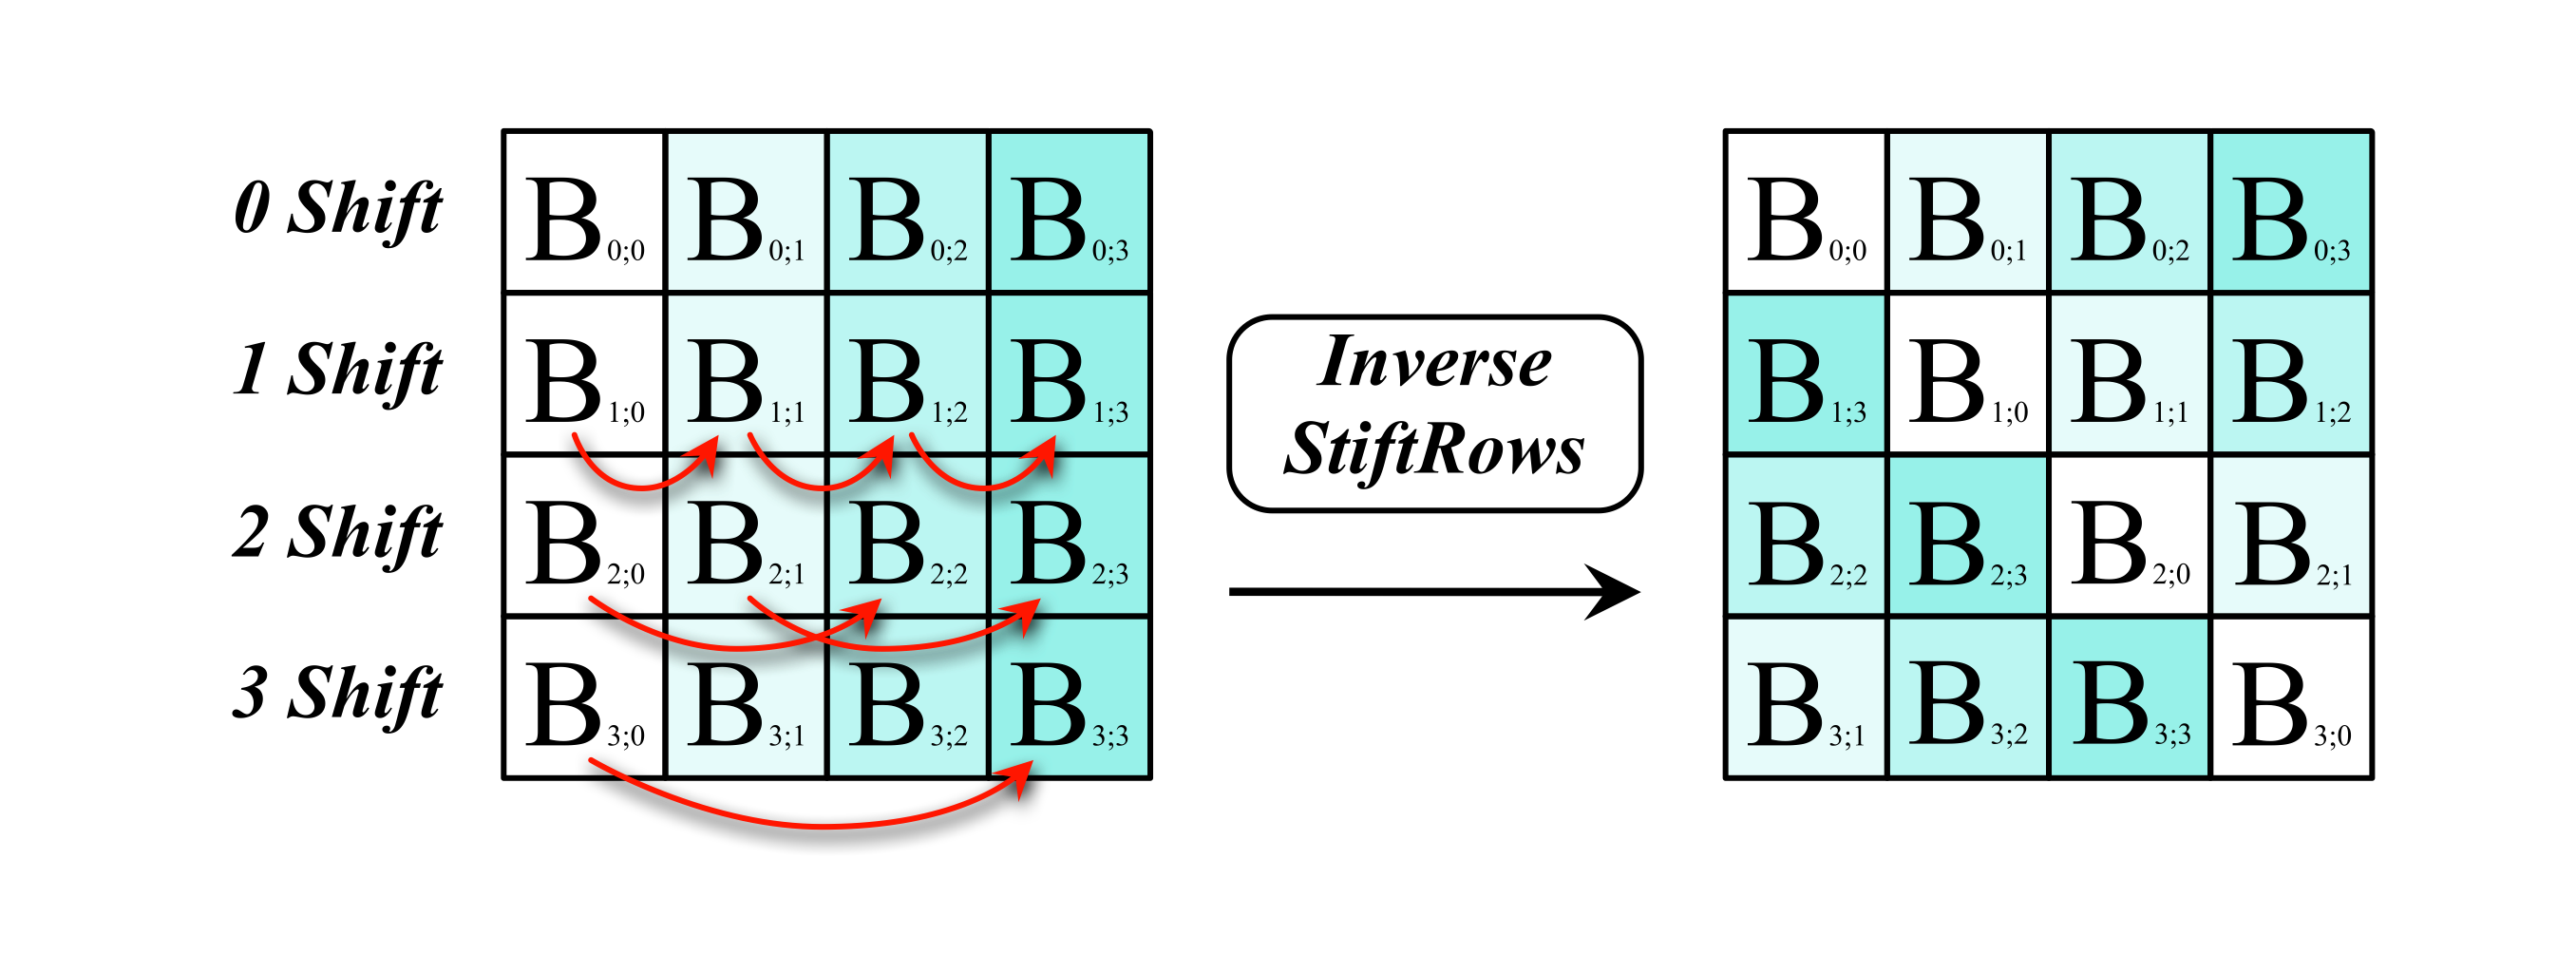
\includegraphics[width=0.7\textwidth]{Inverse-ShiftRows.png}
    \caption{Inverse ShiftRows operationen}
    \label{fig:aes-inverse-shiftrows-pic}
\end{figure}

\subsubsection{MixColumns-operationen}
\label{sec:aes-mixcolumns}

MixColumns-operationen är en operation som primärt agerar på kolumnerna i \gls{byte}-matrisen. Operationen bygger på att varje kolumn multipliceras genom en
\gls{matrismultiplikation} inom \hyperref[sec:finite-fields]{$GF(2^8)$} med en matris som är konstant för alla kolumner. Detta steg gör då att kolumnerna i matrisen omvandlas till nya kolumner,
vilket tillsammans med \nameref{sec:aes-shiftrows} ser till så att inte bara enskilda bytes krypteras utan hela matrisen tillsammans.\footcite{daemen1999aes} Själva operationen visas i figur \ref{fig:aes-mixcolumns-pic}
där även den konstanta matrisen som multipliceras med varje kolumnerna visas.

\begin{figure}[H]
    \centering
    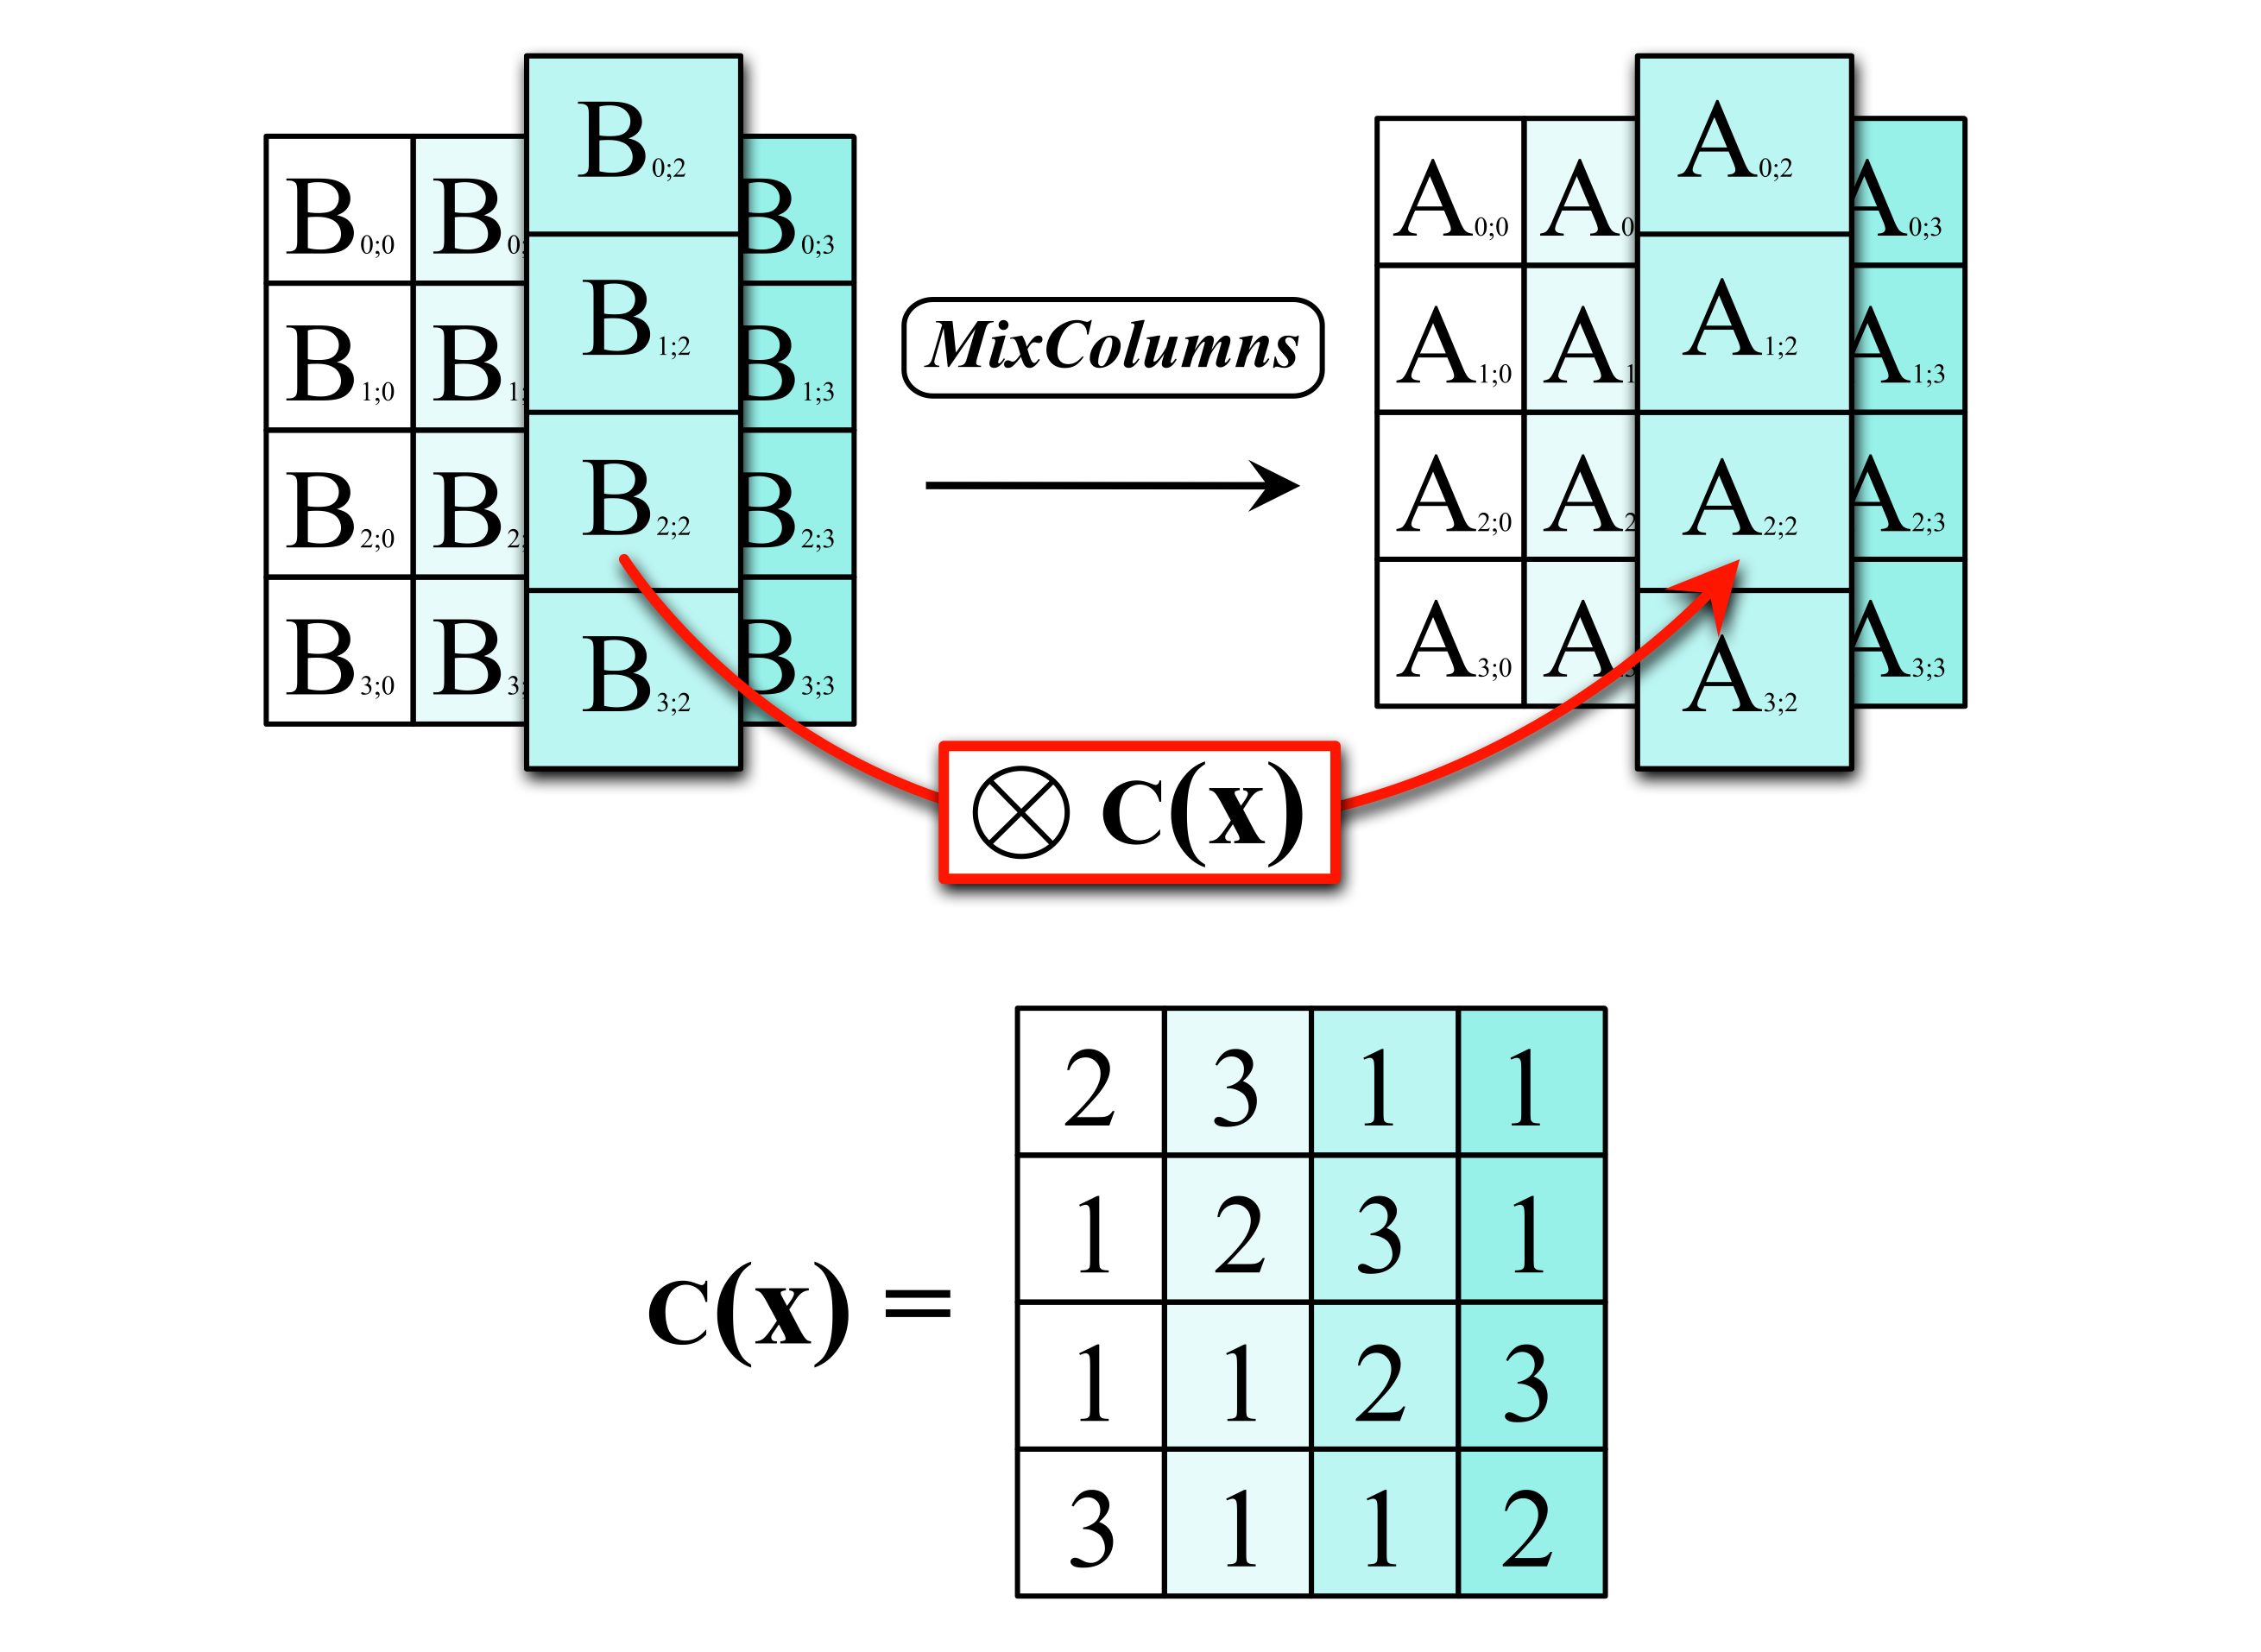
\includegraphics[width=0.7\textwidth]{MixColumns.png}
    \caption{MixColumns operationen}
    \label{fig:aes-mixcolumns-pic}
\end{figure}

\subsubsection{Inverse MixColumns-operationen}
\label{sec:aes-invers-mixcolumns}

Inverse MixColumns-operationen är den motsatta operationen till MixColumns-operationen och fungerar på nästan exakt samma sätt. Operationen bygger på att varje kolumn multipliceras genom en
matrismultiplikation inom \hyperref[sec:finite-fields]{$GF(2^8)$} med en matris som är konstant för alla kolumner. Den stora skillnaden ligger i att den konstanta matrisen som multipliceras med varje kolumn fungerar
som en invers till den tidigare matrisen använd i MixColumns operationen.\footcite{daemen1999aes} Själva operationen visas i figur \ref{fig:aes-inverse-mixcolumns-pic}.

\begin{figure}[H]
    \centering
    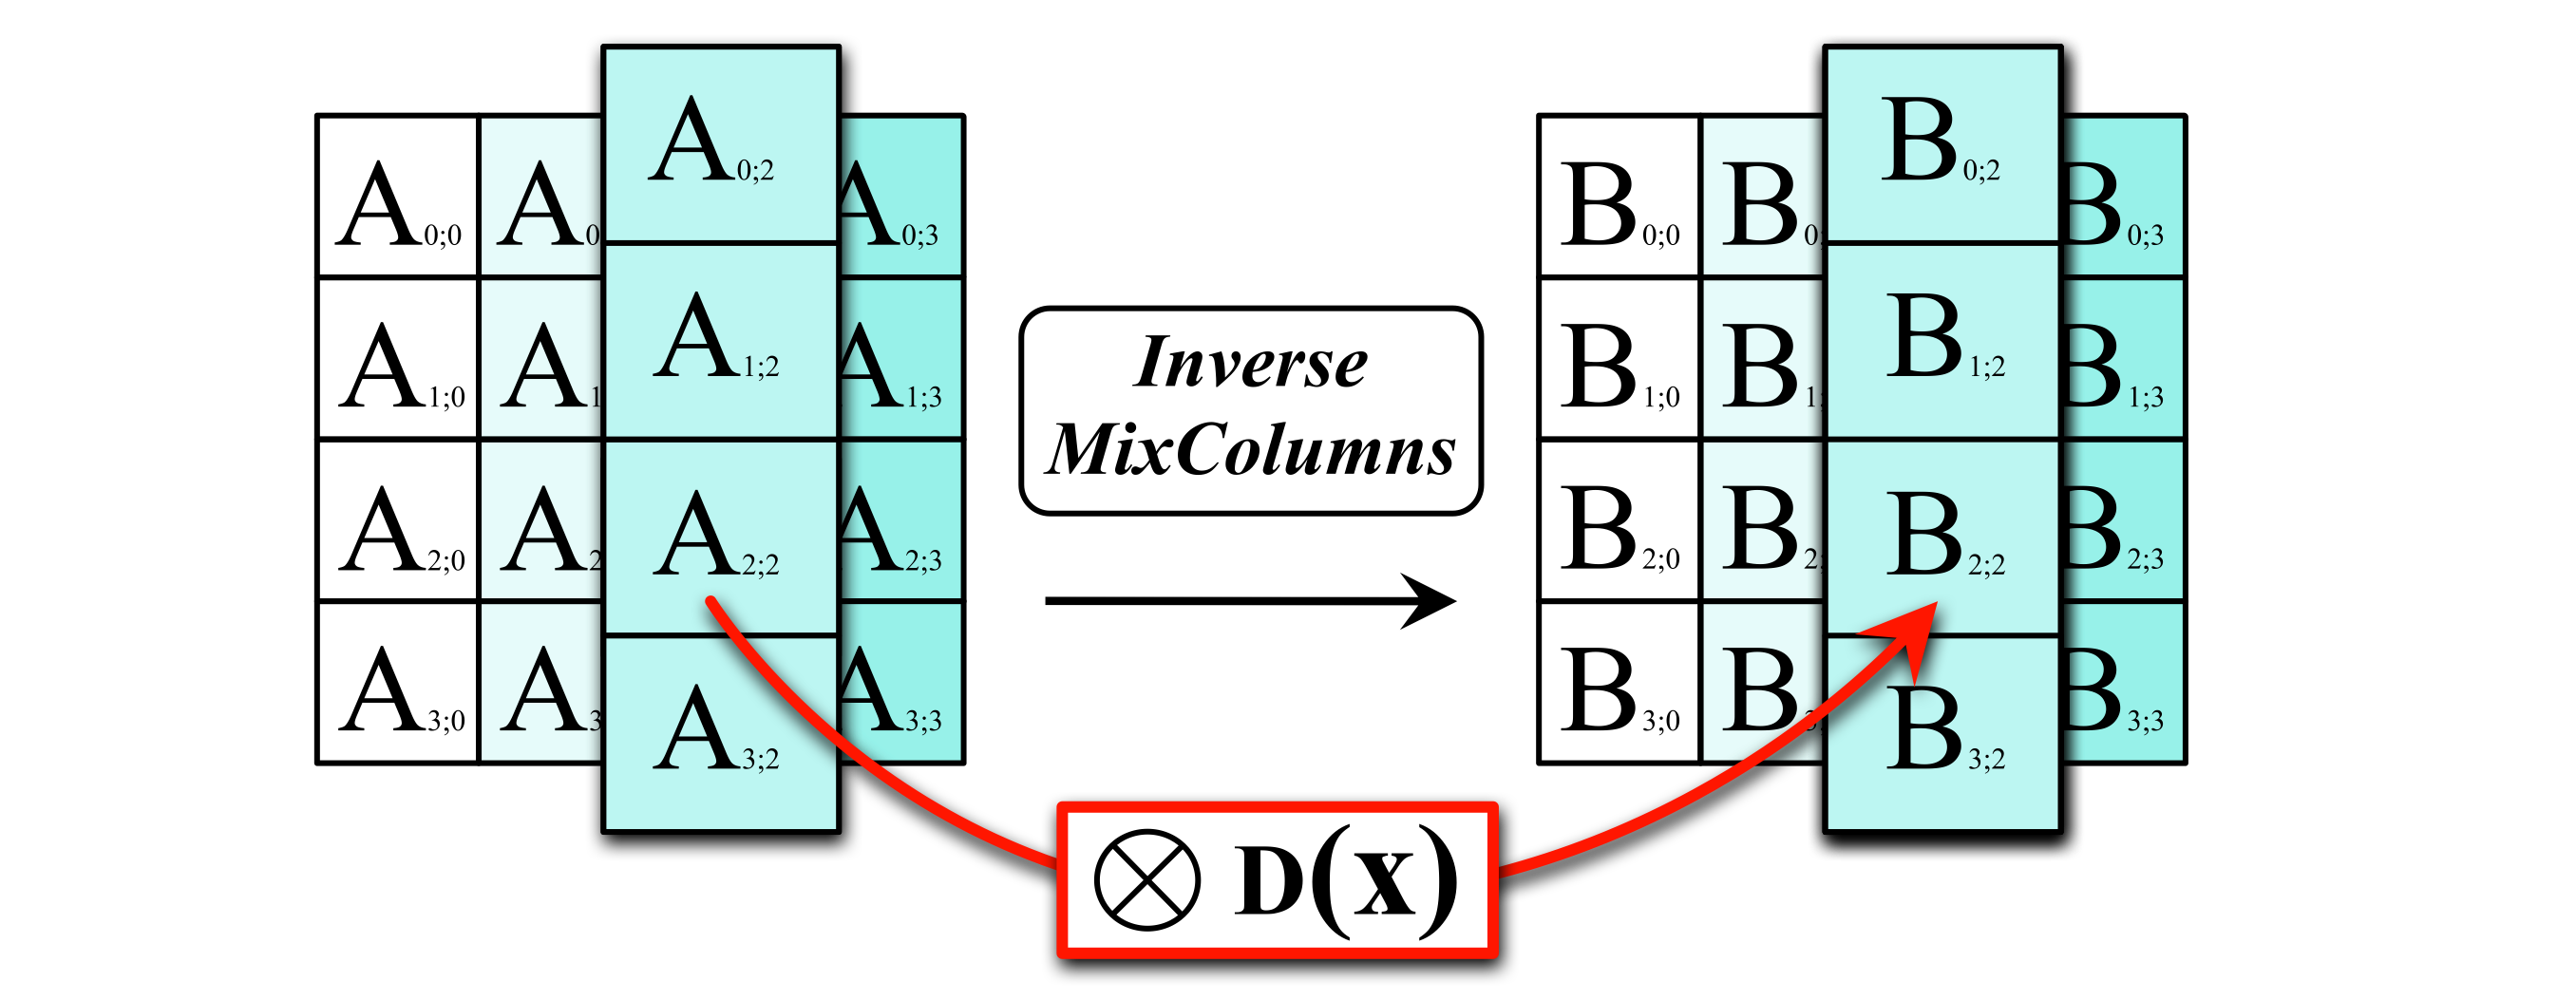
\includegraphics[width=0.7\textwidth]{Inverse-MixColmuns.png}
    \caption{Inverse MixColumns operationen}
    \label{fig:aes-inverse-mixcolumns-pic}
\end{figure}

\subsubsection{AddRoundKey-operationen}
\label{sec:aes-addroundkey}

AddRoundKey-operationen är en operation som bygger på att varje \gls{byte} i \gls{byte}-matrisen genomgår en \gls{xor}-operation med korresponderande \gls{byte} i en nyckelmatris.
I det här steget så introduceras nyckeln i krypteringsprocessen vilket är en viktig del av AES som gör det möjligt att kryptera och dekryptera informationen så länge man har rätt nyckel.\footcite{daemen1999aes}

\begin{figure}[H]
    \centering
    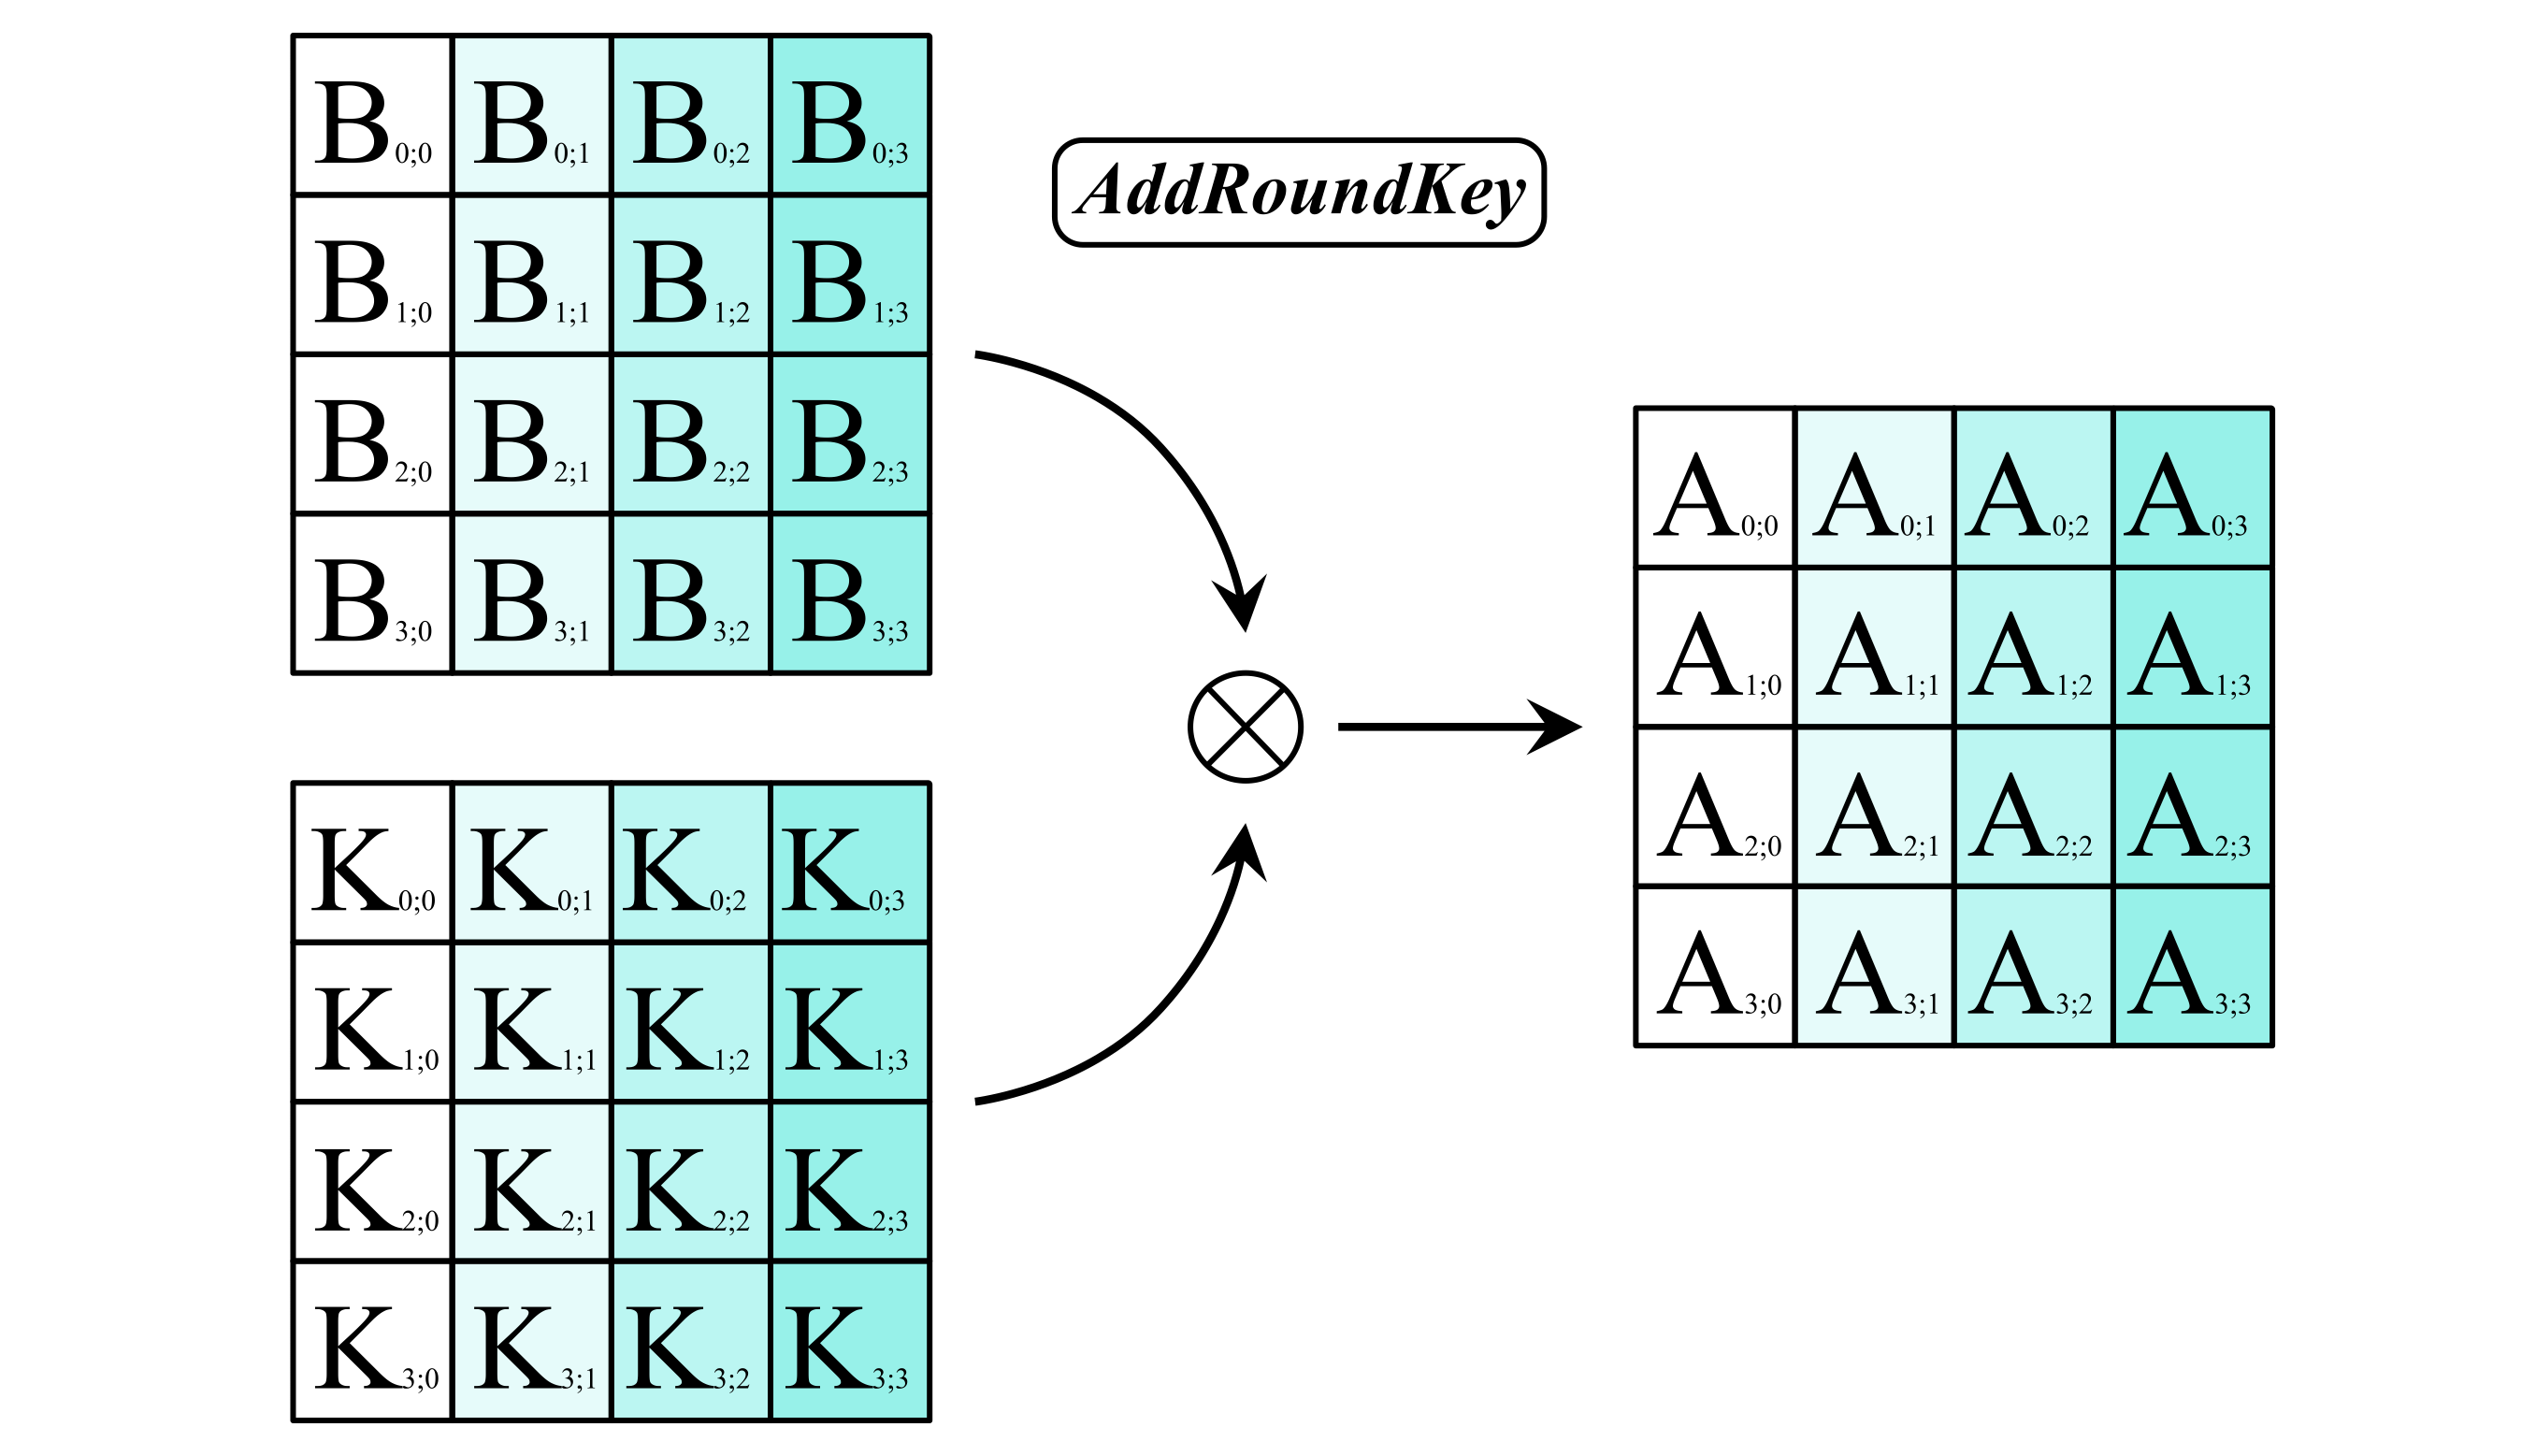
\includegraphics[width=0.7\textwidth]{AddRoundKey.png}
    \caption{AddRoundKey operationen}
    \label{fig:aes-addroundkey-pic}
\end{figure}

\pagebreak
\subsection{Nyckelutökning}
\label{sec:aes-key-expansion}

Nyckelutökningen är den operation som används för att utöka den angivna nyckeln till antingen 11, 13 eller 15 nycklar beroende på längden av den angivna nyckeln.
Anledningen till att antalet nycklar inte är den samma som antalet rundor är för att det innan första rundan genomförs en inledande \nameref{sec:aes-addroundkey} som använder den första nyckeln.
Nyckelutökningen är en viktig del av AES som ser till att det finns en unik nyckel för varje runda i krypteringsprocessen.
Själva utökningen av nyckeln genomförs genom att först dela upp den ursprungliga nyckeln i 4 så kallade words.\footcite{daemen1999aes}

Varje word består av 4 \gls{byte} och är därmed 32 \gls{bit}s långa.
Därefter så genereras varje nytt word utifrån det tidigare worden. Det fyra nästkommande worden genereras genom att ta det sista wordet i den tidigare nyckeln och genom föra en serie av operationer
på detta word. Först så genomförs en \hyperref[sec:aes-rotword]{RotWord}-operation och sedan en \hyperref[sec:aes-subword]{SubWord}-operation samt slutligen en \hyperref[sec:aes-rcon]{Rcon}-operation.\footcite{daemen1999aes}

Därefter så genereras det första wordet i nästa nyckel genom en \gls{xor}-operation mellan det första wordet i den tidigare nyckeln och det resultat som genererades i föregående steg.
Sedan så genereras resterande tre words genom att en \gls{xor}-operation genomförs mellan det tidigare wordet och det koresponderande wordet i den tidigare nyckeln.
Denna process upprepas tills alla nycklar genererats.\footcite{daemen1999aes} Själva processen visas även i figur \ref{fig:aes-key-expansion-pic}.

\begin{figure}[H]
    \centering
    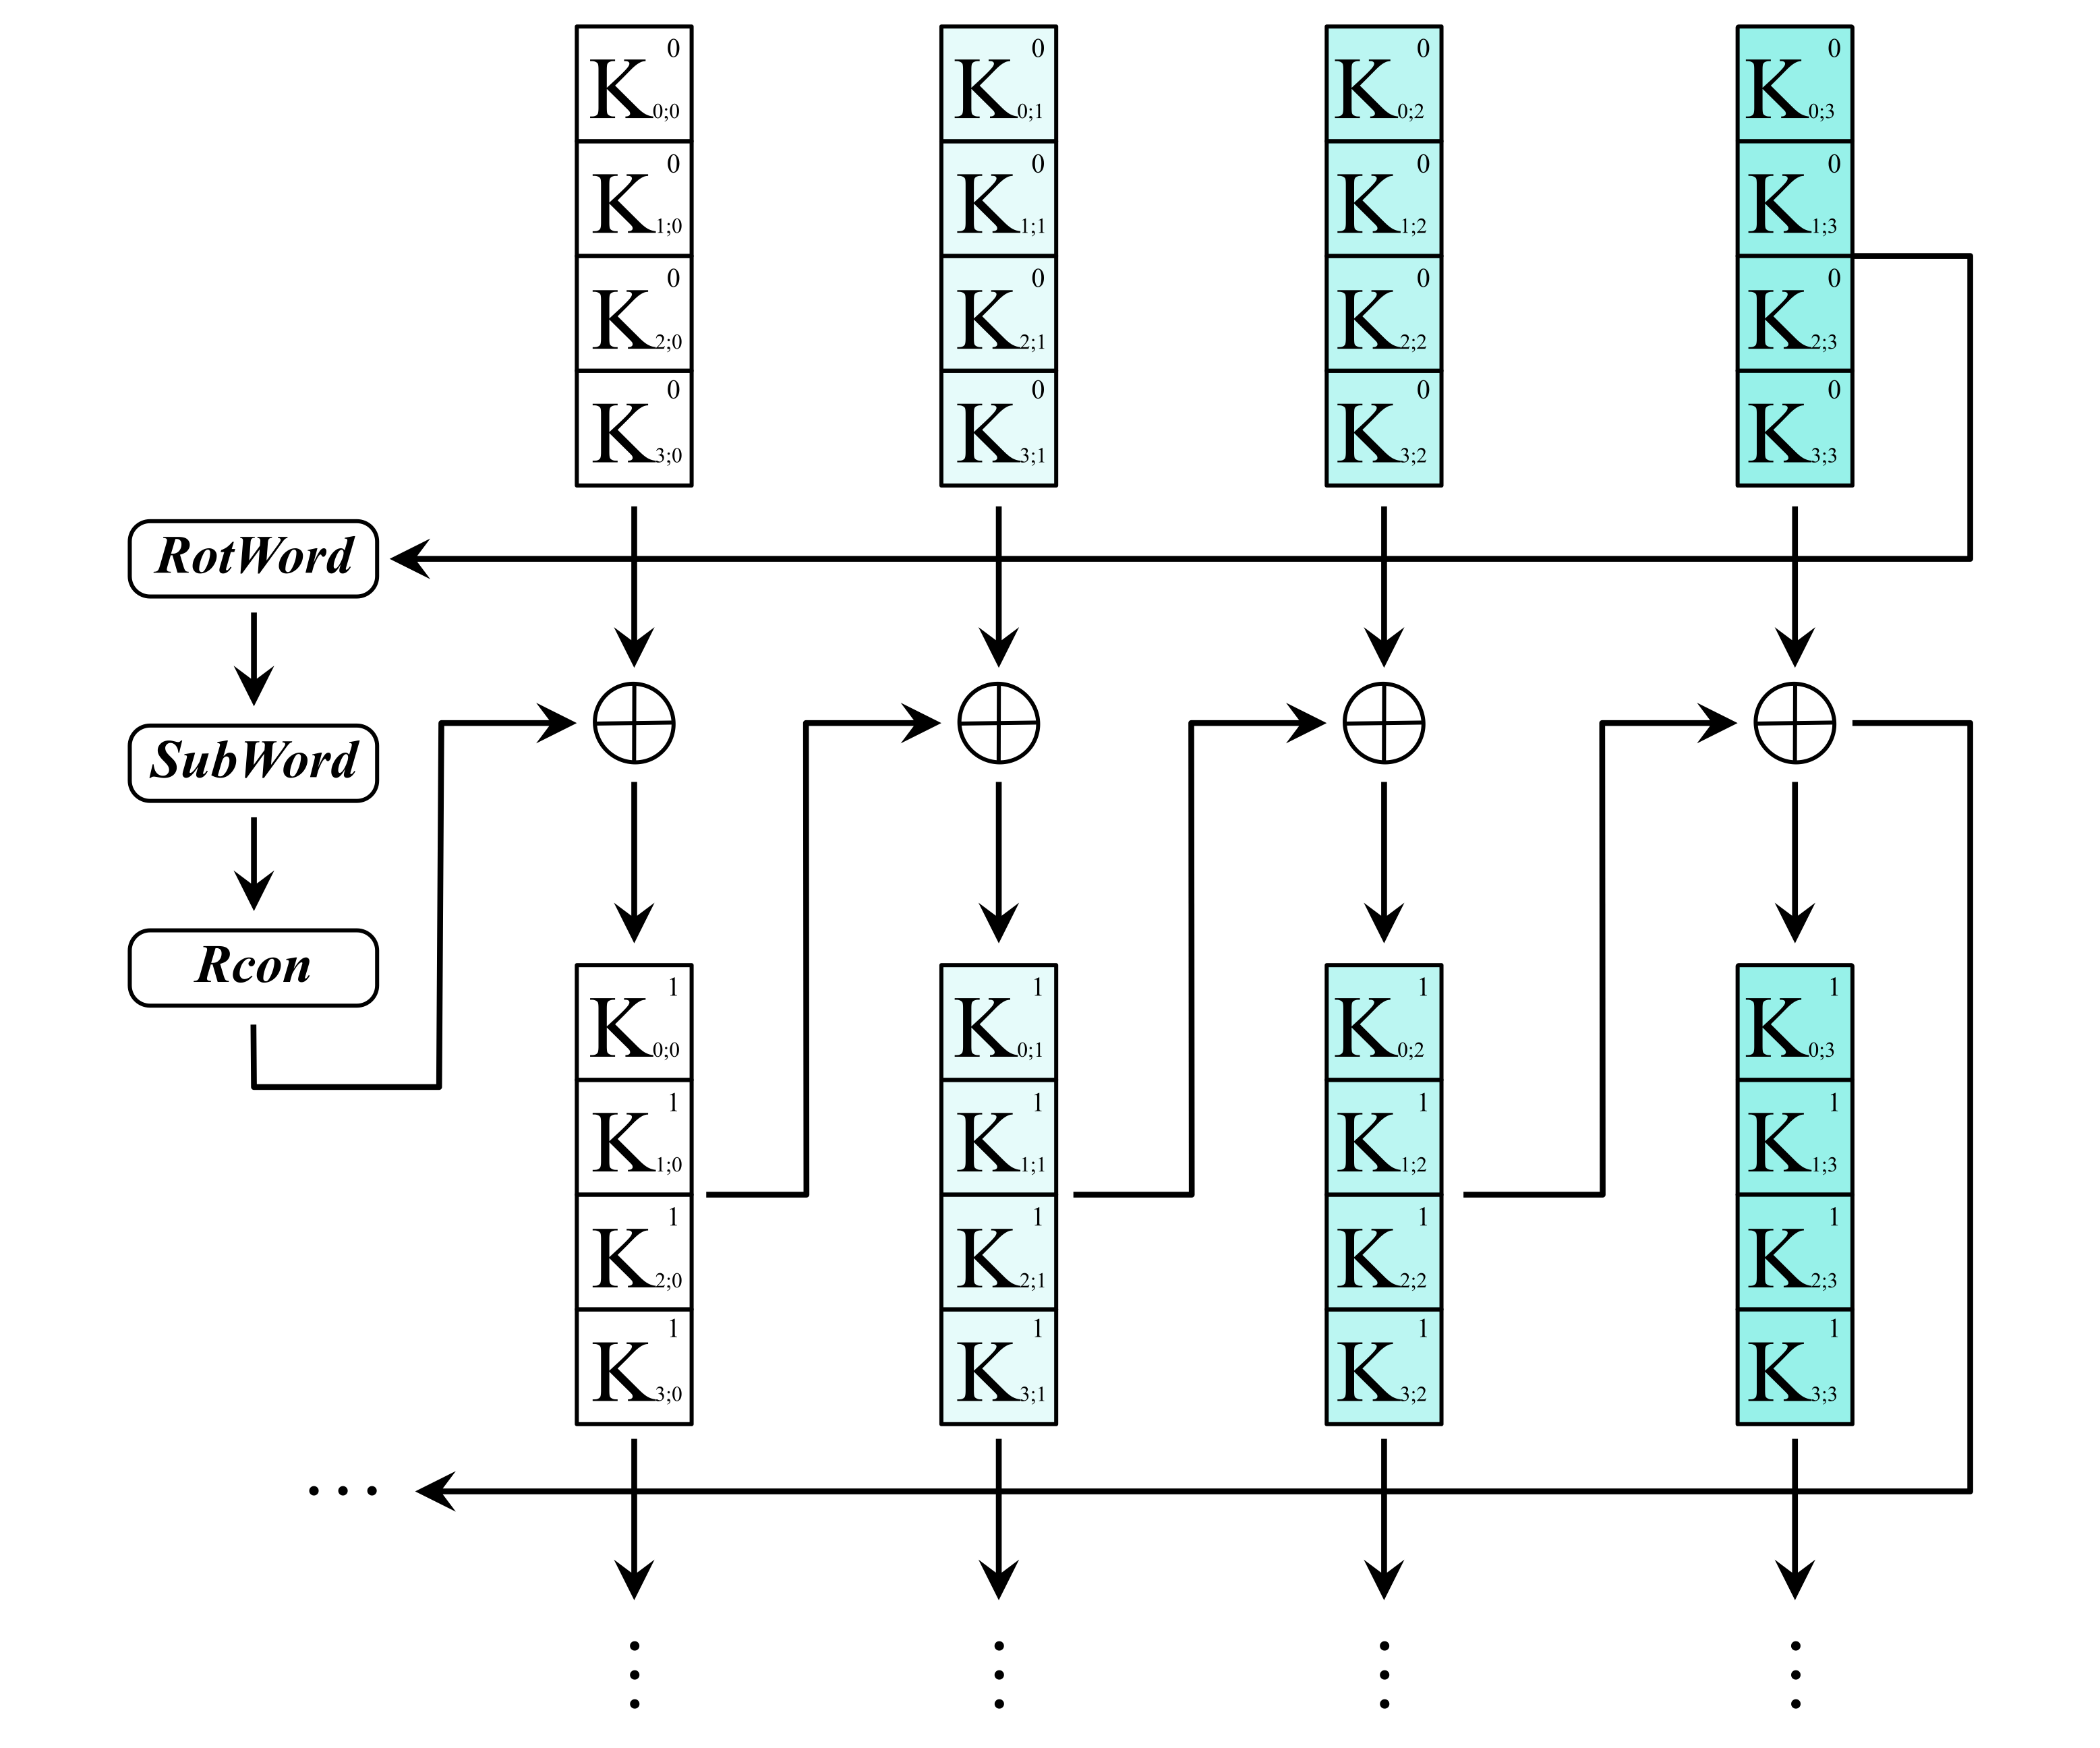
\includegraphics[width=0.8\textwidth]{KeyExpansion.png}
    \caption{Nyckel utöknings processen}
    \label{fig:aes-key-expansion-pic}
\end{figure}

\subsubsection{RotWord}
\label{sec:aes-rotword}

RotWord-operationen är en operation som liknar \nameref{sec:aes-shiftrows} och fungerar så att varje \gls{byte} i wordet skiftas en position till vänster.\footcite{daemen1999aes}
Detta innebär att den första \gls{byte}n i wordet hamnar sist och den sista \gls{byte}n hamnar först, vilket går att se i figur \ref{fig:aes-rotword-pic}.

\begin{figure}[H]
    \centering
    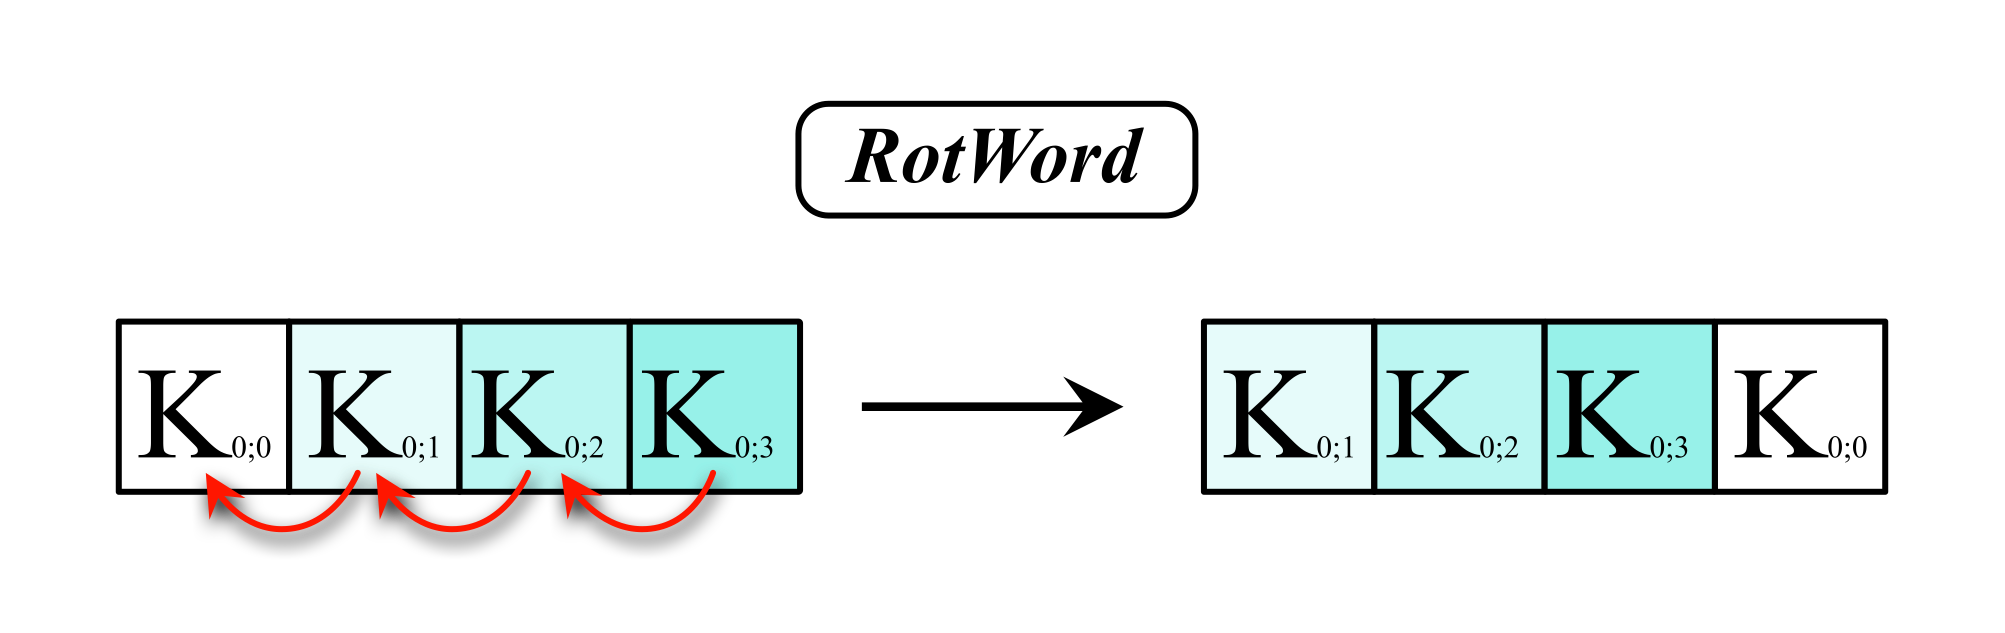
\includegraphics[width=0.7\textwidth]{RotWord.png}
    \caption{RotWord operationen}
    \label{fig:aes-rotword-pic}
\end{figure}

\subsubsection{SubWord}
\label{sec:aes-subword}

SubWord-operationen är en operation som är nästan identisk med \nameref{sec:aes-subbytes}. Själva operationen går ut på att varje \gls{byte} i wordet byts ut mot den korresponderande \gls{byte}n i \nameref{sec:aes-sbox}.\footcite{daemen1999aes}
Som visas i figur \ref{fig:aes-subword-pic}.

\begin{figure}[H]
    \centering
    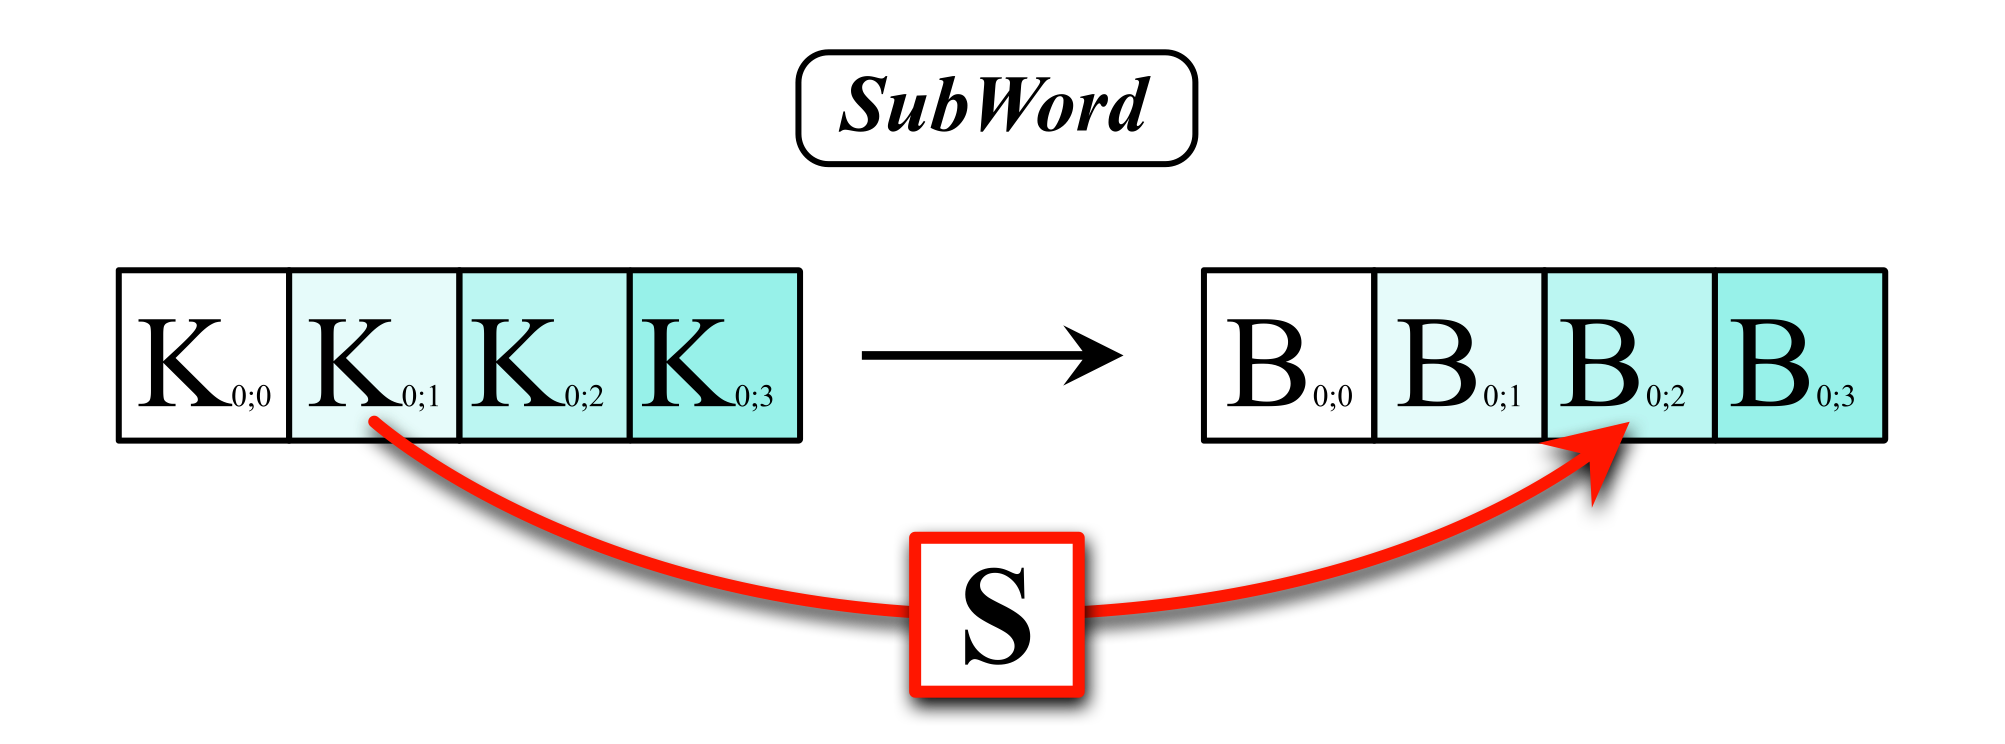
\includegraphics[width=0.7\textwidth]{SubWord.png}
    \caption{SubWord operationen}
    \label{fig:aes-subword-pic}
\end{figure}

\subsubsection{Rcon}
\label{sec:aes-rcon}

\acrshort{rcon}-operationen bygger på att hela wordet genomgår en \gls{xor}-operation med ett speciellt word som är förutbestämt $[rc_i, 0, 0, 0]$, vilket går att se i figur \ref{fig:aes-rcon-pic}.
Det förutbestämda wordet beror vilket nummer nyckeln som genereras är.
Exempelvis ifall det är nyckel nummer 2 så kommer det förutbestämda wordet vara $[1, 0, 0, 0]$. Det ända som förändras beroende på numret på nyckeln är den första \gls{byte}n.\footcite{daemen1999aes}
Värdet på den \gls{byte}n bestäms genom följande regler:

\begin{center}
    \begin{math}
        rc_i =
        \begin{cases}
            1 & \text{ifall } i = 1 \\
            2 \cdot rc_{i-1} & \text{ifall } i > 1 \text{ och } rc_{i-1} < 80_{16} \\
            (2 \cdot rc_{i-1}) \oplus \text {11B}_{16} & \text{ifall } i > 1 \text{ och } rc_{i-1} \ge 80_{16}
        \end{cases}
    \end{math}
\end{center}

Där $\oplus$ är en \gls{xor}-operation, $i$ är vilket nummer på nyckel det är -1 eftersom det första fyra worden är den ursprungliga nyckeln.
Utifrån dessa regler för $rc_i$ så kan man då räkna ut det förutbestämda wordet för varje nyckel som behövs.\footcite{daemen1999aes}

\begin{figure}[H]
    \centering
    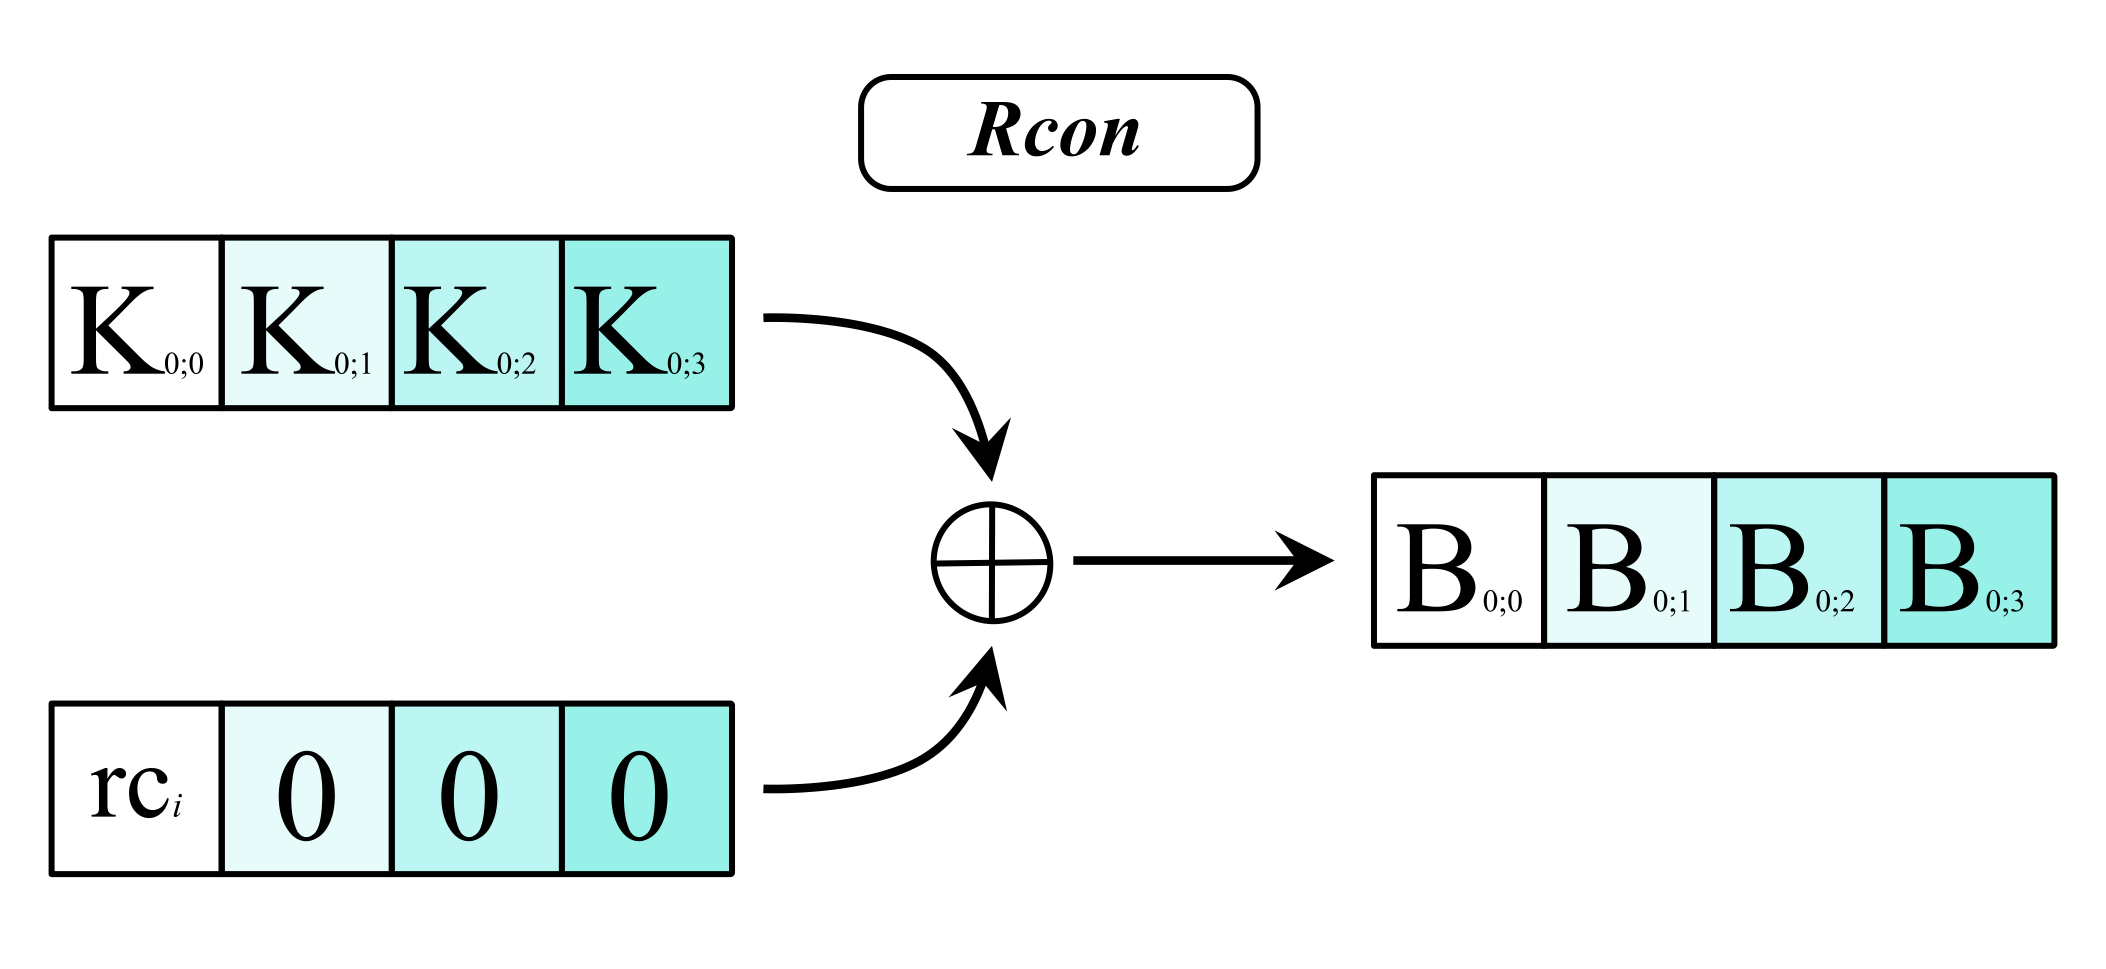
\includegraphics[width=0.7\textwidth]{Rcon.png}
    \caption{Rcon operationen}
    \label{fig:aes-rcon-pic}
\end{figure}
